\section{Details of the $[[20,2,6]]$ $C_4$-Helix code}
\label{apx:code_construction}


Here we provide additional details on the construction of the $[[20,2,6]]$ $C_4$-Helix code and its logical gadgets. We start the CSD construction~\cite{berthusen2025simple} with the well-known $[[5,1,3]]$ non-CSS code~\cite{laflamme1996} with symplectic parity check matrix:
\begin{align}
H_{[[5,1,3]]} =  \left(\begin{array}{c|c}
1 0 0 1 0 & 0 1 1 0 0 \\
0 1 0 0 1 & 0 0 1 1 0 \\
1 0 1 0 0 & 0 0 0 1 1 \\
0 1 0 1 0 & 1 0 0 0 1 
% 0 0 1 0 1 & 1 1 0 0 0
\end{array} \right).
\label{eq:513pcm}
\end{align}
We then obtain the $[[10,2,3]]$ symplectic double code~\cite{burton2024} by considering Eq.~\eqref{eq:513pcm} as $H = (H_X|H_Z)$ and constructing the following parity check matrix
\begin{equation}
\mathfrak{D}(H) = \begin{pmatrix}
\begin{array}{cc|cc}
H_X & H_Z & 0 & 0 \\
0 & 0 & H_Z & H_X \\
\end{array}
\end{pmatrix}.
\label{eq:pcm_double}
\end{equation}
Explicitly, the stabilizer generators and logical operators for the $[[10,2,3]]$ code are shown in the left panel of Table~\ref{tab:codes}, including the two redundant stabilizers resulting from the redundant stabilizer $ZZXIX$ in the $[[5,1,3]]$ code. The stabilizers of the $[[10,2,3]]$ code can be laid out to be planar on a twisted torus, as shown in Fig.~\ref{fig:memory_main}(b). It is for this reason that the $[[10,2,3]]$ code is called a twisted, or cyclic~\cite{Sarkar_2024} Toric code. Measuring the stabilizer generators of the twisted Toric code can be done using the standard ``N-Z" schedule for surface codes~\cite{Tomita_2014}. Projective state preparation must be done with a different stabilizer measurement schedule in order to be fault-tolerant.
% ; this ``cross" schedule is shown by the white, dashed lines in Fig.~\ref{fig:twisted_toric}. 



The symplectic double construction gives the $[[10,2,3]]$ code a ZX-duality~\cite{Breuckmann_2024}, $\tau: \{i, i+5\}_{0,...,9}$. It is along this symmetry that we concatenate with the $[[4,2,2]]$, or $C_4$ code~\cite{Vaidman_1996, Grassl_1997} ,with logical operators defined to be $XIIX$, $IIZZ$, $IIXX$, $ZIIZ$. At a high level, the concatenation procedure can be thought of as replacing each physical qubit of the $[[10,2,3]]$ code with a logical qubit from a $C_4$ codeblock. Physical qubits are assigned to codeblocks according to $\tau$, e.g., physical qubits 0 and 5 are placed in the same $C_4$ codeblock. The assignment of logicals within a $C_4$ codeblock can be arbitrary, but we default to treating the lower indexed physical qubit as the 0th logical qubit. The resulting concatenated code then has two weight-4 generators coming from each of the five $C_4$ codeblocks and eight weight-8 generators obtained by including all $[[10,2,3]]$ stabilizer generators but replacing each single-qubit Pauli operator with the corresponding $C_4$ logical operator, e.g., $X_3$ is replaced with $\overline{X}_0$ on the fourth $C_4$ block---$X_{12}X_{15}$. We have 18 independent stabilizer generators, hence yielding a $[[20,2,6]]$ code. The $[[20,2,6]]$ code is self-dual with $H_X = H_Z$.

The exact stabilizer generators (including two that are redundant) are displayed in the right panel of Table~\ref{tab:codes}. Note that the concatenated stabilizers presented in Table~\ref{tab:codes} for the $[[20,2,6]]$ code are slightly different than what would immediately arise from the CSD construction. Instead, we use a representation where some concatenated generators have been multiplied by a $C_4$ stabilizer generator to facilitate more convenient syndrome extraction; see Section~\ref{apx:syndrome_extraction}.

% \begin{figure}[t]
%     \centering
%     \includegraphics[width=\linewidth]{figures/toric10.png}
%     \caption{\textbf{$C_4$-Helix code schematic. a.} The $[[10,2,3]]$ twisted toric code. Syndrome extraction for both $X-$ and $Z-$type stabilizer generators can be done in parallel with the black ``N-Z" schedule. Projective state preparation can be performed fault-tolerantly by using the white, dashed ``cross" schedule. \textbf{b.} The $[[20,2,6]]$ $C_4$-Helix code. Physical qubits of the twisted toric code are grouped together, e.g. $\{0,5\}$, and replaced with logical qubits of a $[[4,2,2]]$~\cite{Vaidman_1996, Knill_1998} code.
%     \drew{Recommend to make some combined version of a,b part of Fig 1 instead of the Torus}
%     }
%     \label{fig:twisted_toric}
% \end{figure}




% \clearpage
\begin{table*}
% \centering

\begin{minipage}{0.33\textwidth}
\raggedleft
\begin{tabular}{cccccccccccc}
0 & 1 & 2 & 3 & 4 & 5 & 6 & 7 & 8 & 9 & \\
\hline
$X$& $\cdot$& $\cdot$& $X$& $\cdot$& $\cdot$& $X$& $X$& $\cdot$& $\cdot$&\\
$\cdot$& $X$& $\cdot$& $\cdot$& $X$& $\cdot$& $\cdot$& $X$& $X$& $\cdot$&\\
$X$& $\cdot$& $X$& $\cdot$& $\cdot$& $\cdot$& $\cdot$& $\cdot$& $X$& $X$&\\
$\cdot$& $X$& $\cdot$& $X$& $\cdot$& $X$& $\cdot$& $\cdot$& $\cdot$& $X$&\\
$\cdot$& $\cdot$& $X$& $\cdot$& $X$& $X$& $X$& $\cdot$& $\cdot$& $\cdot$&\\
\hline
$\cdot$& $Z$& $Z$& $\cdot$& $\cdot$& $Z$& $\cdot$& $\cdot$& $Z$& $\cdot$&\\
$\cdot$& $\cdot$& $Z$& $Z$& $\cdot$& $\cdot$& $Z$& $\cdot$& $\cdot$& $Z$&\\
$\cdot$& $\cdot$& $\cdot$& $Z$& $Z$& $Z$& $\cdot$& $Z$& $\cdot$& $\cdot$&\\
$Z$& $\cdot$& $\cdot$& $\cdot$& $Z$& $\cdot$& $Z$& $\cdot$& $Z$& $\cdot$&\\
$Z$& $Z$& $\cdot$& $\cdot$& $\cdot$& $\cdot$& $\cdot$& $Z$& $\cdot$& $Z$&\\
\hline
$\cdot$& $\cdot$& $X$& $X$& $\cdot$& $X$& $\cdot$& $\cdot$& $\cdot$& $\cdot$& $=X_0$\\
$X$& $\cdot$& $\cdot$& $\cdot$& $\cdot$& $\cdot$& $X$& $\cdot$& $\cdot$& $X$& $=X_1$\\
$\cdot$& $Z$& $\cdot$& $\cdot$& $Z$& $Z$& $\cdot$& $\cdot$& $\cdot$& $\cdot$& $=Z_0$\\
$Z$& $\cdot$& $\cdot$& $\cdot$& $\cdot$& $\cdot$& $\cdot$& $Z$& $Z$& $\cdot$& $=Z_1$\\
\end{tabular}
% \caption*{[[10,2,3]] code}
\end{minipage}
\hfill
\begin{minipage}{0.6\textwidth}
\raggedright
\begin{tabular}{cccccccccccccccccccccc}
0 & 1 & 2 & 3 & 4 & 5 & 6 & 7 & 8 & 9 & 10 & 11 & 12 & 13 & 14 & 15 & 16 & 17 & 18 & 19 & \\
\hline
$X$& $X$& $X$& $X$& $\cdot$& $\cdot$& $\cdot$& $\cdot$& $\cdot$& $\cdot$& $\cdot$& $\cdot$& $\cdot$& $\cdot$& $\cdot$& $\cdot$& $\cdot$& $\cdot$& $\cdot$& $\cdot$&\\
$\cdot$& $\cdot$& $\cdot$& $\cdot$& $X$& $X$& $X$& $X$& $\cdot$& $\cdot$& $\cdot$& $\cdot$& $\cdot$& $\cdot$& $\cdot$& $\cdot$& $\cdot$& $\cdot$& $\cdot$& $\cdot$&\\
$\cdot$& $\cdot$& $\cdot$& $\cdot$& $\cdot$& $\cdot$& $\cdot$& $\cdot$& $X$& $X$& $X$& $X$& $\cdot$& $\cdot$& $\cdot$& $\cdot$& $\cdot$& $\cdot$& $\cdot$& $\cdot$&\\
$\cdot$& $\cdot$& $\cdot$& $\cdot$& $\cdot$& $\cdot$& $\cdot$& $\cdot$& $\cdot$& $\cdot$& $\cdot$& $\cdot$& $X$& $X$& $X$& $X$& $\cdot$& $\cdot$& $\cdot$& $\cdot$&\\
$\cdot$& $\cdot$& $\cdot$& $\cdot$& $\cdot$& $\cdot$& $\cdot$& $\cdot$& $\cdot$& $\cdot$& $\cdot$& $\cdot$& $\cdot$& $\cdot$& $\cdot$& $\cdot$& $X$& $X$& $X$& $X$&\\
$X$& $\cdot$& $\cdot$& $X$& $\cdot$& $\cdot$& $X$& $X$& $\cdot$& $\cdot$& $X$& $X$& $X$& $\cdot$& $\cdot$& $X$& $\cdot$& $\cdot$& $\cdot$& $\cdot$&\\
$\cdot$& $\cdot$& $\cdot$& $\cdot$& $X$& $\cdot$& $\cdot$& $X$& $X$& $X$& $\cdot$& $\cdot$& $\cdot$& $\cdot$& $X$& $X$& $X$& $\cdot$& $\cdot$& $X$&\\
$\cdot$& $X$& $X$& $\cdot$& $\cdot$& $\cdot$& $\cdot$& $\cdot$& $X$& $\cdot$& $\cdot$& $X$& $X$& $X$& $\cdot$& $\cdot$& $\cdot$& $\cdot$& $X$& $X$&\\
$\cdot$& $\cdot$& $X$& $X$& $\cdot$& $X$& $X$& $\cdot$& $\cdot$& $\cdot$& $\cdot$& $\cdot$& $\cdot$& $X$& $X$& $\cdot$& $X$& $X$& $\cdot$& $\cdot$&\\
$X$& $X$& $\cdot$& $\cdot$& $X$& $X$& $\cdot$& $\cdot$& $\cdot$& $X$& $X$& $\cdot$& $\cdot$& $\cdot$& $\cdot$& $\cdot$& $\cdot$& $X$& $X$& $\cdot$&\\
\hline
$Z$& $Z$& $Z$& $Z$& $\cdot$& $\cdot$& $\cdot$& $\cdot$& $\cdot$& $\cdot$& $\cdot$& $\cdot$& $\cdot$& $\cdot$& $\cdot$& $\cdot$& $\cdot$& $\cdot$& $\cdot$& $\cdot$&\\
$\cdot$& $\cdot$& $\cdot$& $\cdot$& $Z$& $Z$& $Z$& $Z$& $\cdot$& $\cdot$& $\cdot$& $\cdot$& $\cdot$& $\cdot$& $\cdot$& $\cdot$& $\cdot$& $\cdot$& $\cdot$& $\cdot$&\\
$\cdot$& $\cdot$& $\cdot$& $\cdot$& $\cdot$& $\cdot$& $\cdot$& $\cdot$& $Z$& $Z$& $Z$& $Z$& $\cdot$& $\cdot$& $\cdot$& $\cdot$& $\cdot$& $\cdot$& $\cdot$& $\cdot$&\\
$\cdot$& $\cdot$& $\cdot$& $\cdot$& $\cdot$& $\cdot$& $\cdot$& $\cdot$& $\cdot$& $\cdot$& $\cdot$& $\cdot$& $Z$& $Z$& $Z$& $Z$& $\cdot$& $\cdot$& $\cdot$& $\cdot$&\\
$\cdot$& $\cdot$& $\cdot$& $\cdot$& $\cdot$& $\cdot$& $\cdot$& $\cdot$& $\cdot$& $\cdot$& $\cdot$& $\cdot$& $\cdot$& $\cdot$& $\cdot$& $\cdot$& $Z$& $Z$& $Z$& $Z$&\\
$Z$& $\cdot$& $\cdot$& $Z$& $\cdot$& $\cdot$& $Z$& $Z$& $\cdot$& $\cdot$& $Z$& $Z$& $Z$& $\cdot$& $\cdot$& $Z$& $\cdot$& $\cdot$& $\cdot$& $\cdot$&\\
$\cdot$& $\cdot$& $\cdot$& $\cdot$& $Z$& $\cdot$& $\cdot$& $Z$& $Z$& $Z$& $\cdot$& $\cdot$& $\cdot$& $\cdot$& $Z$& $Z$& $Z$& $\cdot$& $\cdot$& $Z$&\\
$\cdot$& $Z$& $Z$& $\cdot$& $\cdot$& $\cdot$& $\cdot$& $\cdot$& $Z$& $\cdot$& $\cdot$& $Z$& $Z$& $Z$& $\cdot$& $\cdot$& $\cdot$& $\cdot$& $Z$& $Z$&\\
$\cdot$& $\cdot$& $Z$& $Z$& $\cdot$& $Z$& $Z$& $\cdot$& $\cdot$& $\cdot$& $\cdot$& $\cdot$& $\cdot$& $Z$& $Z$& $\cdot$& $Z$& $Z$& $\cdot$& $\cdot$&\\
$Z$& $Z$& $\cdot$& $\cdot$& $Z$& $Z$& $\cdot$& $\cdot$& $\cdot$& $Z$& $Z$& $\cdot$& $\cdot$& $\cdot$& $\cdot$& $\cdot$& $\cdot$& $Z$& $Z$& $\cdot$&\\
\hline
$\cdot$& $\cdot$& $X$& $X$& $\cdot$& $\cdot$& $\cdot$& $\cdot$& $X$& $\cdot$& $\cdot$& $X$& $X$& $\cdot$& $\cdot$& $X$& $\cdot$& $\cdot$& $\cdot$& $\cdot$& $=X_0$\\
$X$& $\cdot$& $\cdot$& $X$& $\cdot$& $\cdot$& $X$& $X$& $\cdot$& $\cdot$& $\cdot$& $\cdot$& $\cdot$& $\cdot$& $\cdot$& $\cdot$& $\cdot$& $\cdot$& $X$& $X$& $=X_1$\\
$Z$& $\cdot$& $\cdot$& $Z$& $\cdot$& $\cdot$& $Z$& $Z$& $\cdot$& $\cdot$& $\cdot$& $\cdot$& $\cdot$& $\cdot$& $\cdot$& $\cdot$& $\cdot$& $\cdot$& $Z$& $Z$& $=Z_0$\\
$\cdot$& $\cdot$& $Z$& $Z$& $\cdot$& $\cdot$& $\cdot$& $\cdot$& $Z$& $\cdot$& $\cdot$& $Z$& $Z$& $\cdot$& $\cdot$& $Z$& $\cdot$& $\cdot$& $\cdot$& $\cdot$& $=Z_1$\\
\end{tabular}
% \caption*{[[20,2,6]] code}
\end{minipage}

\caption{\textbf{Stabilizers and logical operators for the [[10,2,3]] and [[20,2,6]] codes.}}
\label{tab:codes}
\end{table*}


\begin{figure*}
    \centering
    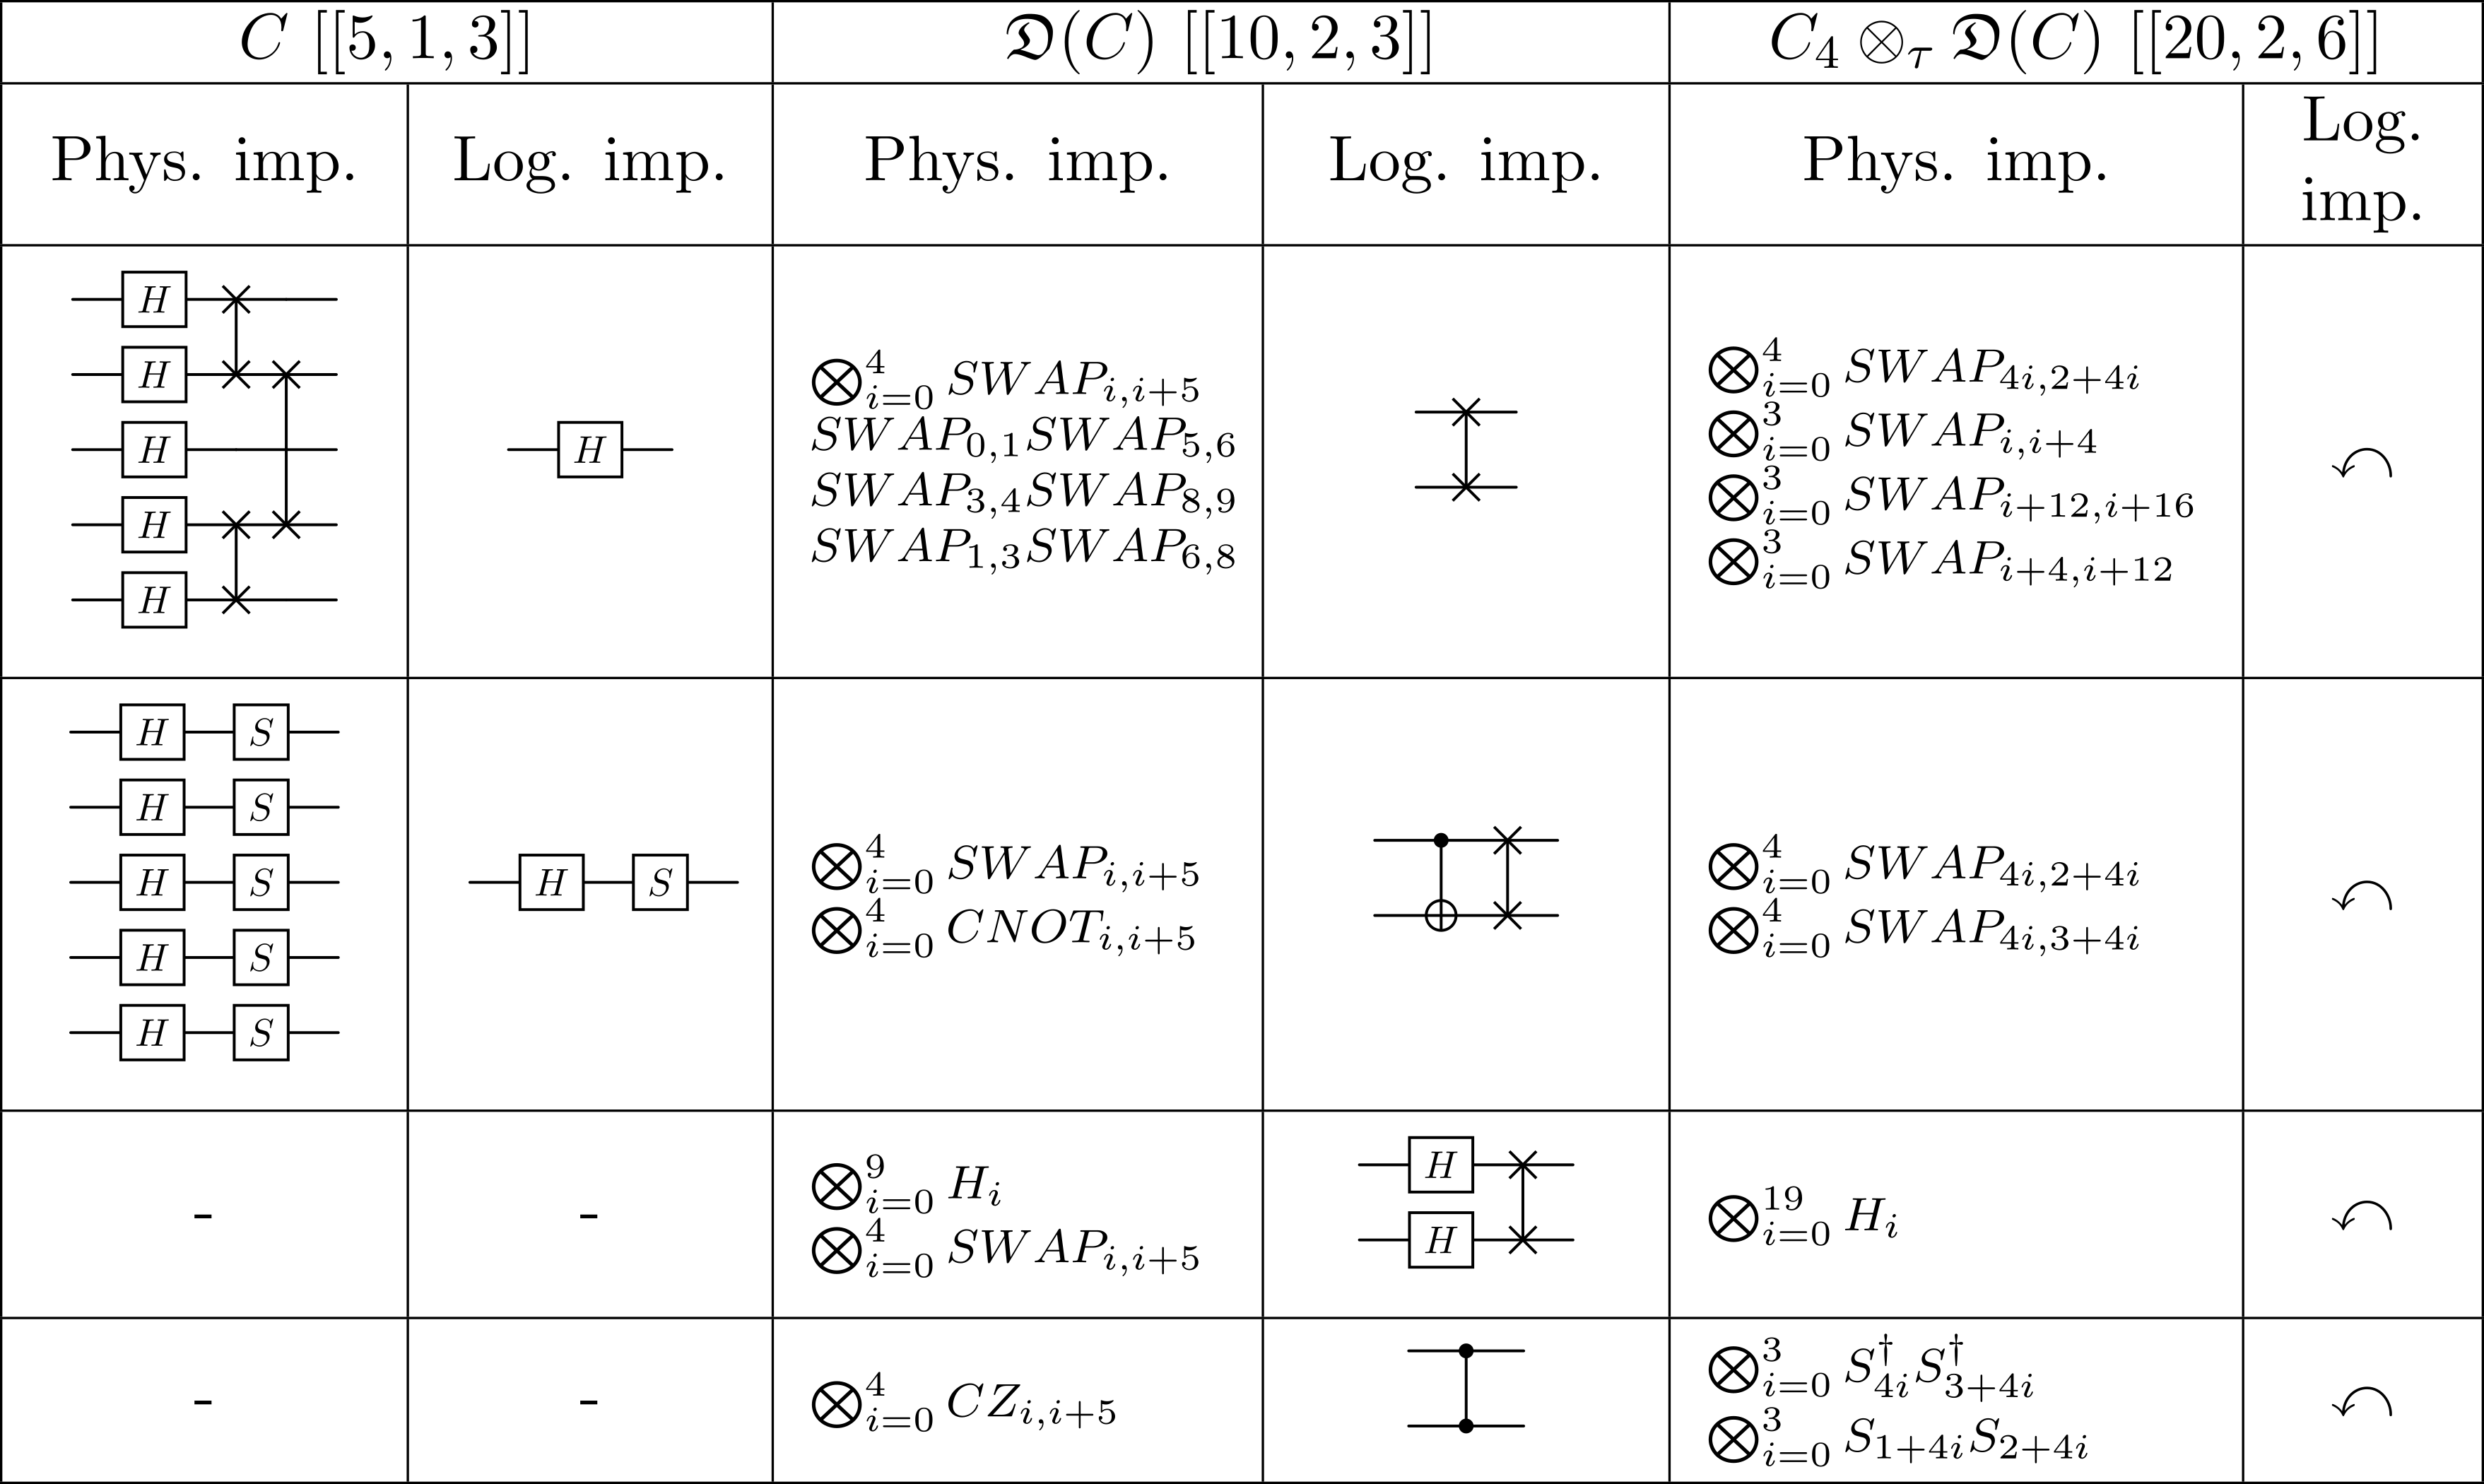
\includegraphics[width=0.83\linewidth]{figures/table.png}
    \caption{\textbf{Logical gates for the $C_4$-Helix code sequence}. SWAP-transversal gates on the non-CSS $[[5,1,3]]$ code lifting to SWAP- and fold-transversal logical gates on the $[[10,2,3]]$ symplectic double code, lifting again to SWAP-transversal gates on the $[[20,2,6]]$ CSD code.}
    \label{fig:actions}
\end{figure*}


\subsection{Logical Clifford gates}

The symplectic double and CSD constructions yield codes with many fold-transversal and SWAP-transversal (automorphism) gates, respectively, see Section 3.1 of Ref.~\cite{berthusen2025simple} for complete details. We list the available gates for the sequence of codes $[[5,1,3]] \rightarrow [[10,2,3]] \rightarrow [[20,2,6]]$ in Fig.~\ref{fig:actions}. Two gates come from lifting the $\overline{H}$ and $\overline{H} \overline{S}$ logical gates available on the $[[5,1,3]]$ code, while the H-SWAP and CZ-S gates~\cite{Breuckmann_2024} arise from the ZX-duality on the $[[10,2,3]]$ code. All of these gates are automorphisms on the $[[20,2,6]]$ code, and as such can be implemented using only single-qubit gates and qubit relabeling in software. These automorphism gates, $G$, generate a group of size $|G| = 36$. 

To complete the two-qubit symplectic group, where $|\rm{Sp}_4(\mathbb{F}_2)| = 720$, an additional logical gate is required. We choose to implement a global $S$ gate, $\overline{S}_0 \overline{S}_1$. In Ref.~\cite{berthusen2025simple} it was suggested to realize this gate through gate injection~\cite{Zhou2000} during quantum error correction; however, the overheads of doing so are prohibitive, especially on near-term hardware. Instead, we consider an optimization-based approach~\cite{kuehnke2025} to search for gates implementing $\overline{S}_0\overline{S}_1$ on the $[[10,2,3]]$ code. We choose a gate that lifts nicely when implemented on the logical qubits of the five $[[4,2,2]]$ codeblocks; it and its lifted version are shown in Fig.~\ref{fig:ft_phase_gate}(a), (c). Unfortunately, due to the intra-block physical CZ gates, the circuit in Fig.~\ref{fig:ft_phase_gate}(c) is not immediately fault-tolerant. To remedy this, we replace each physical CZ gate with the flag gadget~\cite{Chao_2018} depicted in Fig.~\ref{fig:ft_phase_gate}(b). We verify with Stim~\cite{Gidney_2021} that, when followed by syndrome extraction, the circuit-level distance of this $\overline{S}_0\overline{S}_1$ gate is 6. Note that, as described, the logical global phase gate actually implements $\overline{S}_0 \overline{S}_1 \overline{Z}_0 \overline{Z}_1$ and the logical CZ gate actually implements $\overline{CZ}_{0,1} \overline{Z}_1$. While these actions are correct in the symplectic sense, it is required to determine if there are residual Paulis when implementing some two-qubit logical Clifford operation.









\begin{figure}
    \centering
    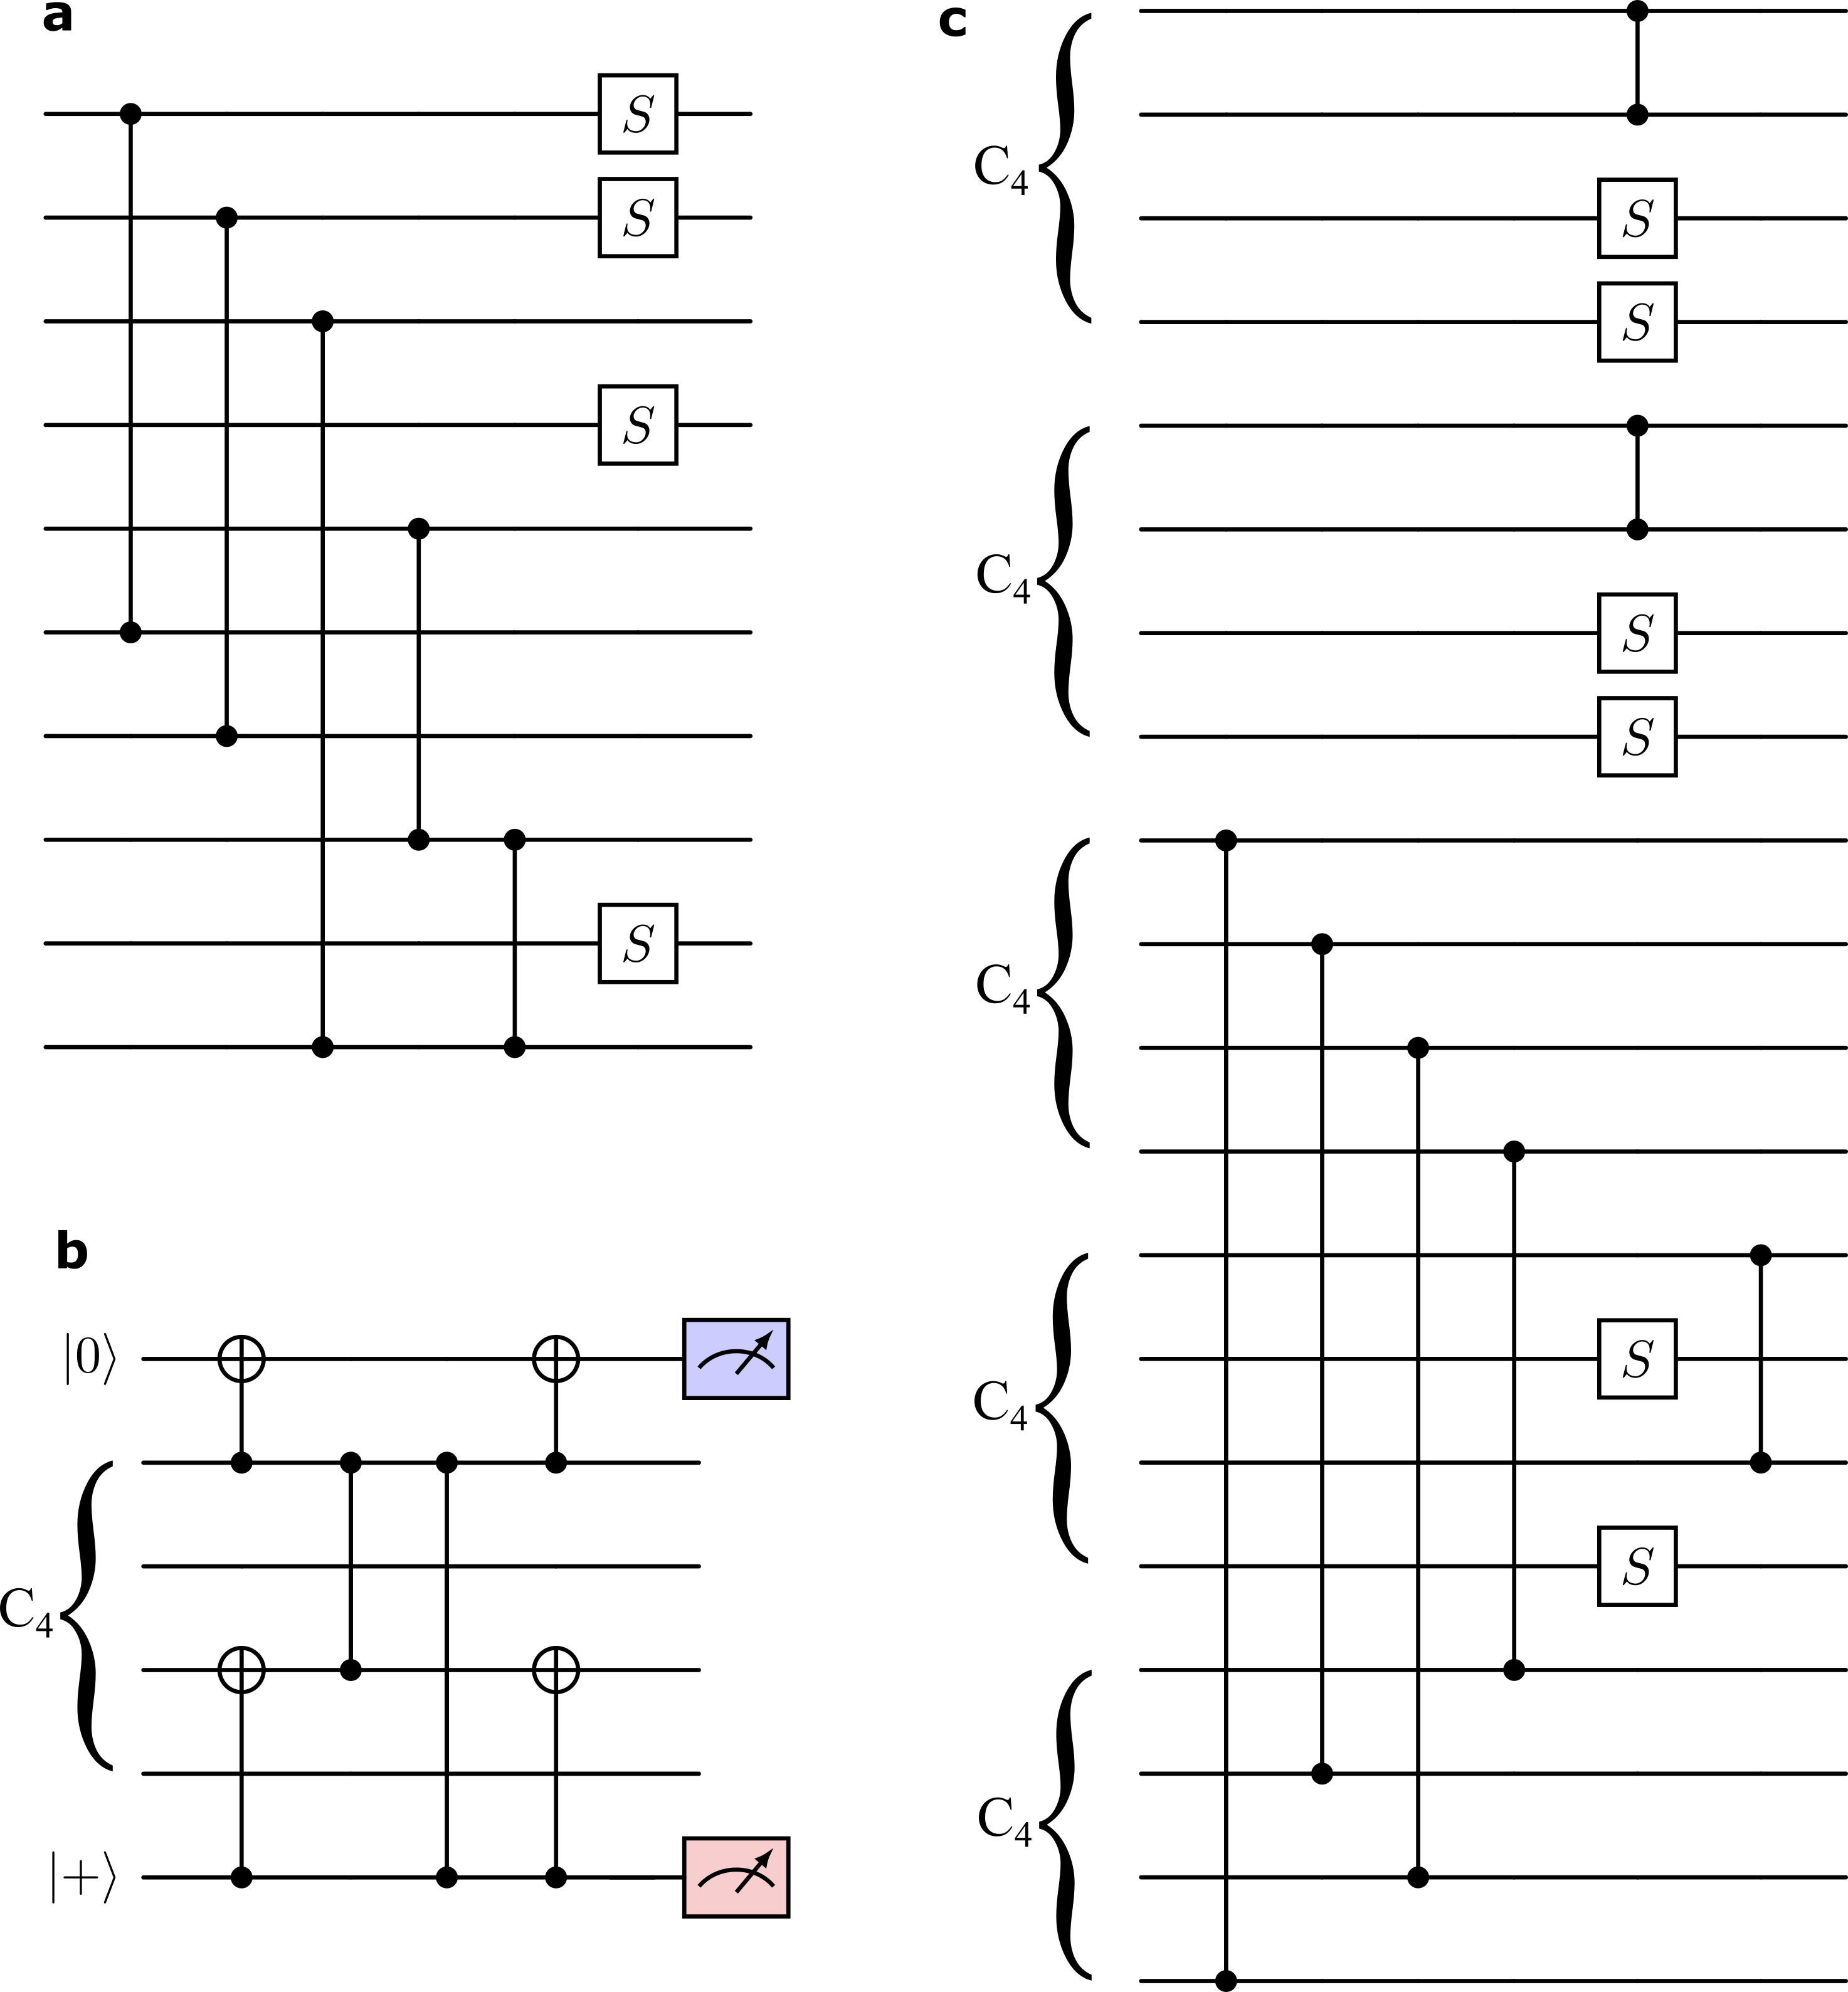
\includegraphics[width=\linewidth]{figures/ft_phase_gate.png}
    \caption{\textbf{Logical phase gates. a.} Implementation of $\overline{S}_0 \overline{S}_1$ on the $[[10,2,3]]$ symplectic double code. \textbf{c.} Non-fault-tolerant implementation of $\overline{S}_0 \overline{S}_1$ on the $[[20,2,6]]$ CSD code. All physical $CZ$ operations are not immediately fault-tolerant, even if followed by QEC. These operations are made fault-tolerant using the flag gadget shown in panel \textbf{b} and following with a round of QEC. }
    \label{fig:ft_phase_gate}
\end{figure}

\begin{figure}
    \centering
    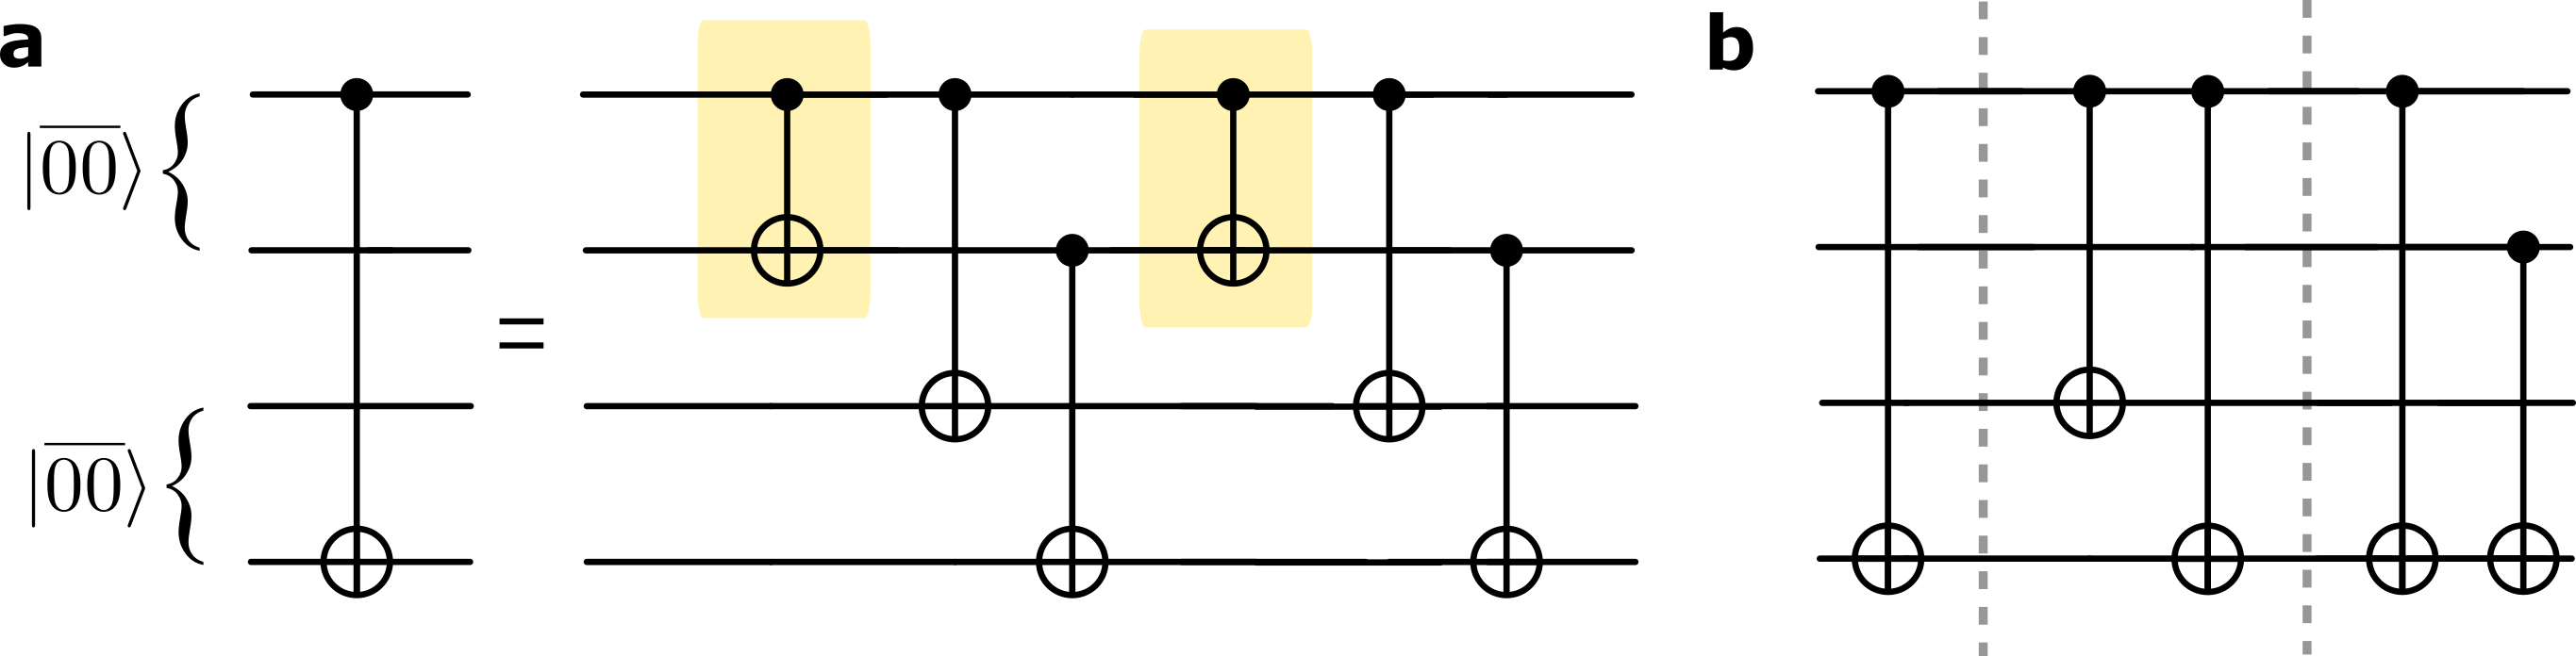
\includegraphics[width=\linewidth]{figures/cnot_circuit.png}
    \caption{\textbf{Targeted interblock CNOT gate. a.} Circuit to implement a targeted inter-block CNOT gate using only transversal CNOT and automorphism gates (highlighted in yellow). \textbf{b.} Available inter-block gates via chain maps~\cite{benhemou2026}. Each gate/gate sequence (separated by a dashed line) can be implemented in depth-2 with a circuit-level distance of 6. Conjugating by SWAP gates in both/either codeblock further increases the available operations.}
    \label{fig:cnot-circuit}
\end{figure}


We can express any element of the two qubit symplectic group (and hence the full Clifford group by including transversal logical Pauli gates) with a sequence of gates from $G$ interleaved with the $\overline{S}_0 \overline{S}_1$ gate. Finding a valid sequence of logical generators then reduces to a word factorization problem in $\rm{Sp}_{2k}(\mathbb{F}_2)$. For arbitrary $k$, this is intractable to solve efficiently; fortunately, we can brute force search over $\rm{Sp}_4(\mathbb{F}_2)$ for factorizations that are optimal in the number of applied $\overline{S}_0 \overline{S}_1$ gates. We do this by performing Dijkstra's algorithm on a Cayley graph of $\rm{Sp}_4(\mathbb{F}_2)$ in which edges representing the global phase gate are assigned a nonzero cost and all other edges---corresponding to the free automorphism gates---have zero cost. Hence the optimal path through the graph is the one utilizing the fewest global phase gates. We then compute the shortest path between the identity and each element of $\rm{Sp}_4(\mathbb{F}_2)$ to build a lookup-table logical compiler. One such compiled Clifford is shown in Fig.~\ref{fig:clifford_bench_main}(d). The maximum number of global phase gates needed to implement an arbitrary two-qubit logical Clifford is three, and the full distribution is 0: 36, 1: 324, 2: 324, 3: 36.


Adding transversal inter-block CNOT gates to $G$ and $\overline{S}_0\overline{S}_1$ is sufficient to generate the full Clifford group on an arbitrary number of codeblocks. One important circuit identity that allows us to implement targeted inter-block CNOT gates is shown in Fig.~\ref{fig:cnot-circuit}(a). Alternatively, we can realize the CNOT circuits in Fig.~\ref{fig:cnot-circuit}(b) using fault-tolerant, depth-2 chain maps found using an automated chain map discovery tool~\cite{benhemou2026}. While the depths are the same between two methods, two rounds of error correction are required for the transversal approach---one after each transversal CNOT gate---whereas, only a single round of error correction is required following the chain map. Hence the cost of realizing inter-code operations via chain maps is effectively half that of the transversal approach; even larger savings are available when implementing logical FANIN/FANOUT gates. An arbitrary $m$-block Clifford operator is compiled into the $C_4$-Helix gateset by first expressing it in terms of inter-block CNOT/CZ gates (targeted and transversal) and intra-block Clifford operators, $U_i \in \mathcal{C}_2$ on each $C_4$-Helix codeblock. These $U_i$'s can then be expressed in terms of the logical generators. This process is illustrated in Fig.~\ref{fig:clifford_bench_main}(a)-(d). It may be possible to first recompile the circuit in such a way that expensive inter-block CNOT gates are minimized. Compiling an arbitrary $m$-block Clifford+T circuit can be done similarly, with the addition that non-Clifford gates also flush the accumulation of any intra-block Clifford operators.

\begin{figure}
    \centering
    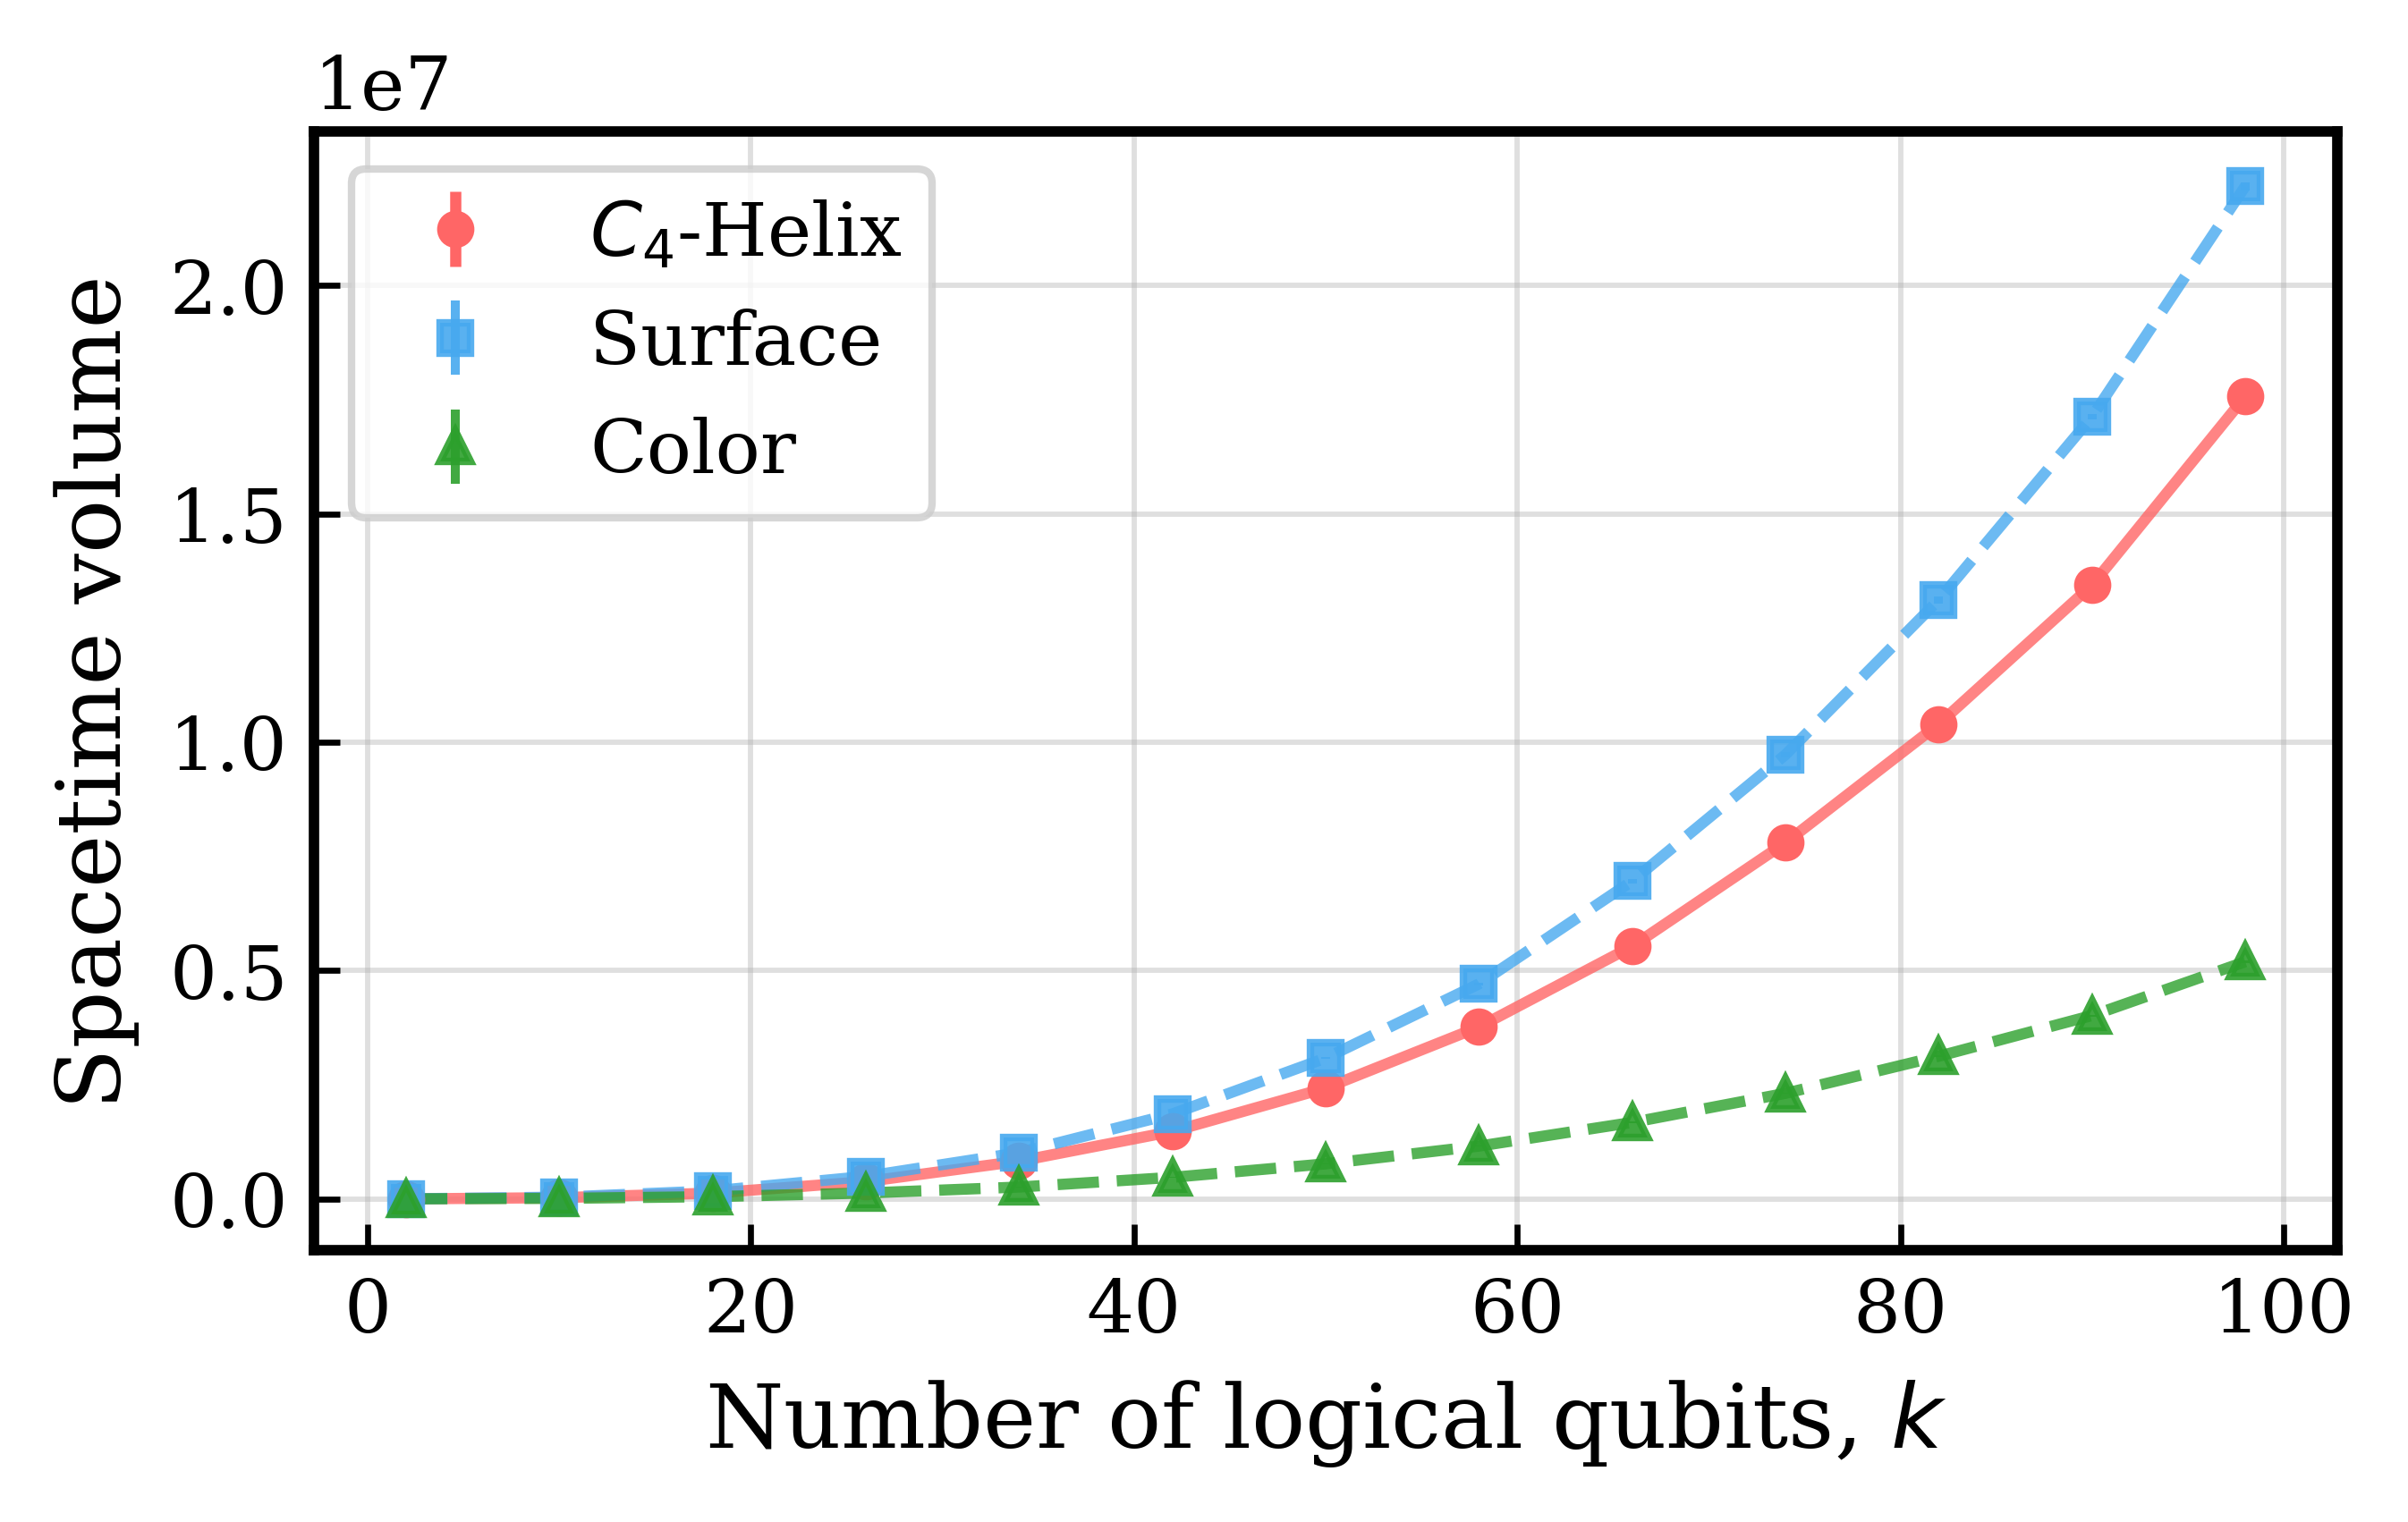
\includegraphics[width=0.95\linewidth]{figures/clifford_bench.png}
    \caption{\textbf{Spacetime volume versus problem size}. Spacetime volume (mean compiled logical depth times number of physical qubits required to encode $k$ logical qubits) of uniformly random $k$-qubit Clifford operators, comparing the $C_4$-Helix gateset, the surface code, and the color code. Each operator is sampled uniformly at random and synthesized into a minimal physical-gate circuit, whose layers are then costed by the native operations of each architecture. Note that syndrome extraction overhead is not considered in this analysis. }
    \label{fig:cliff_bench}
\end{figure}


To illustrate the efficient logical compilation afforded by the $C_4$-Helix gateset, we compile uniformly random $k$-qubit Clifford operators and compare the resulting logical circuit depth against surface code and color code implementations of the same operators. For each qubit count, we sample random Clifford operators, synthesize a minimal physical-gate representation, and cost each layer according to the native operations of the respective architecture: inter-block CNOTs and intra-block $\mathcal{C}_2$ operators (via the lookup-table compiler) for the $C_4$-Helix code, fully transversal, depth-1 gates for the color code, and transversal gates---save for the depth-4 $S$ gate~\cite{chen2026}---for the rotated surface code. As shown in Fig.~\ref{fig:cliff_bench}, the $C_4$-Helix code, despite encoding $k>1$ logical qubits, achieves a spacetime volume (compiled depth times number of physical qubits) that beats the $d=5$ surface code and maintains a small constant factor between the color code. We again emphasize that uniformly random Clifford operators represent a worst-case workload for the $C_4$-Helix code. In practice, quantum algorithms can be compiled to rely predominantly on its inexpensive transversal and automorphism gates, avoiding the costly single-block Clifford and targeted inter-block CNOT operations that dominate the random-circuit cost. As such, the overhead reported here is an upper bound; for structured algorithms the practical cost would fall well below these values, substantially narrowing the gap with the surface and color codes.~\cite{LeBlond2026InPrep}.



\subsection{Syndrome extraction}
\label{apx:syndrome_extraction}

We use different syndrome extraction circuits to measure the stabilizer generators from different levels of concatenation: in a full syndrome extraction round, we first measure the lower-level, weight-$4$ stabilizers in parallel using the circuits shown in Fig.~\ref{fig:se_circuit}(a)-(b). We then measure the upper-level, weight-$8$ $X$-type stabilizers followed by the upper-level, weight-8 $Z$-type stabilizers using the circuit shown in Fig.~\ref{fig:se_circuit}(c). We use $32$ ancillas to parallelize the syndrome extraction as much as possible, resulting in a depth-$10$ circuit for measuring a complete set of $18$ stabilizers. 

To measure the lower-level stabilizer generators of the $C_4$ codeblocks, we use a circuit similar to Ref.~\cite{reichardt2025}, as shown in Fig.~\ref{fig:se_circuit}(a). It uses two ancilla qubits to measure the $X$- and $Z$-type stabilizer of a $C_4$ block in parallel. Each ancilla also acts as a flag qubit for the other ancilla to catch potential hook errors. Lastly, it swaps out two data qubits for the two fresh ancilla qubits, mitigating the effect of leakage on data qubits~\cite{aliferis2007fault, suchara2015leakage}. To ensure all data qubits get swapped out, we alternate between two slightly different circuits (see Fig.~\ref{fig:se_circuit}(b)), where the difference is that they swap out different qubits of the $C_4$ code. By doing so, all data qubits get swapped out after two rounds of syndrome extraction. Since different lower-level $C_4$ blocks are supported on different physical qubits, all lower-level stabilizer can easily be measured in parallel. To measure the upper-level, weight-$8$ $X$-type stabilizers, we use the circuit shown in Fig.~\ref{fig:se_circuit}(c), which uses four ancilla qubits (one syndrome qubit plus three flag qubits) per stabilizer and has CNOT depth of $6$. It is possible to find a schedule to measure all four weight-$8$ $X$-type checks in parallel. Since the code is self-dual, the circuit for measuring the corresponding $Z$-type checks can be obtained by simply reversing the direction of CNOTs and modifying the initialization and measurement bases for ancilla qubits accordingly. 

Since we have enough ancilla qubits at our disposal, we use different ancillas for measuring the upper-level $X$- and $Z$-type stabilizers; this allows us to start the $Z$ syndrome measurement circuits before the $X$ syndrome measurement circuits have finished and hence lower the total depth. Moreover, the upper-level $X$ syndrome extraction circuit can start before the lower-level syndrome extraction circuit has finished to further lower the total depth to 10. 

\begin{figure}[t]
    \centering
    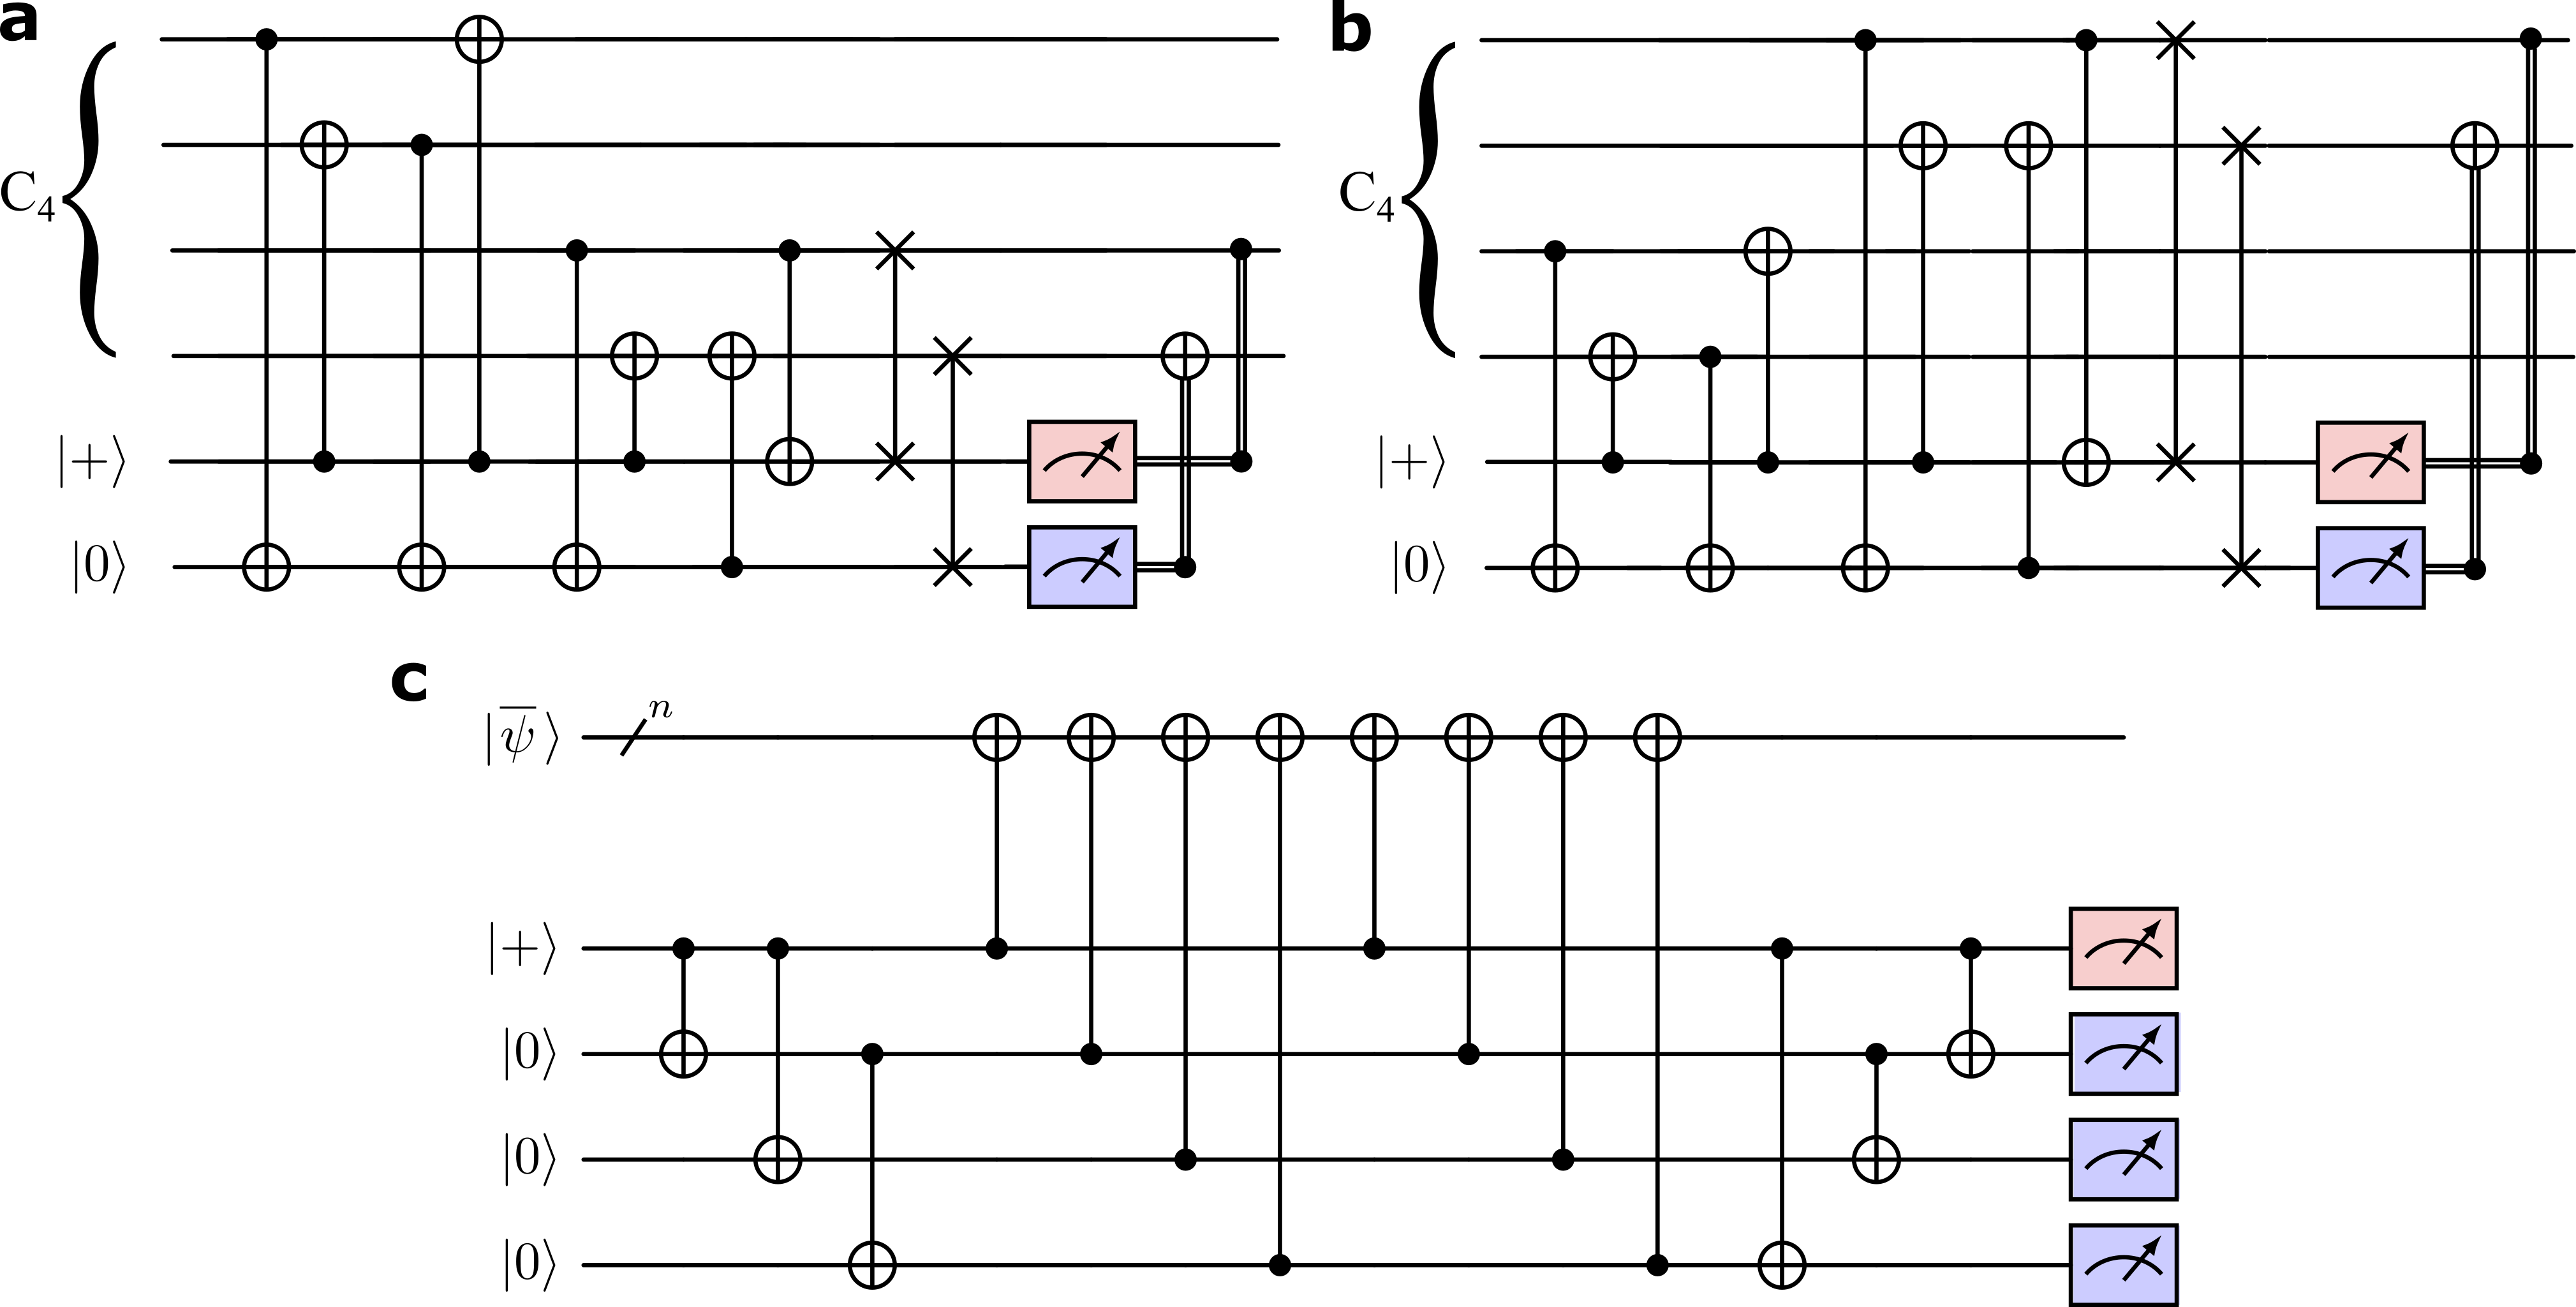
\includegraphics[width=\linewidth]{figures/new_se_circuit.png}
    \caption{\textbf{Syndrome extraction circuits for the $C_4$-Helix code.} \textbf{a.} Circuit to measure the two stabilizer generators of the $C_4$ code. In order to mitigate the effects of leakage, each syndrome extraction round swaps out two data qubits for two fresh ancilla qubits; hence all four data qubits are exchanged every two rounds by alternating the circuits in panels \textbf{a} and \textbf{b}. The SWAP gates drawn are implemented virtually through qubit relabeling and do not introduce additional error. \textbf{c.} Modified Shor-style syndrome extraction for a single weight-8 stabilizer generator. }
    \label{fig:se_circuit}
\end{figure}

\subsubsection{Adaptive syndrome extraction}
\label{section:ase}

Since the $C_4$-Helix code is a concatenated code with the $C_4$ code as the lower code, we can readily apply adaptive syndrome extraction (ASE)~\cite{Berthusen_2025} to reduce spacetime overheads and consequently lower logical error rates. In the original prescription of ASE, the stabilizer generators of the lower $C_4$ codeblocks were first measured, then only concatenated generators that shared support with a triggered $C_4$ generator are measured. For the $C_4$-Helix code, each $C_4$ generator overlaps with four out of the five concatenated generators coming from the twisted toric code. Measuring the exact set of overlapping generators adds complexity to implementation and decoding, see below, that is likely not worth the slight reduction in gate count. As such, we make the simplification that if any of the $C_4$ stabilizer generators indicate that an error has occurred, all ten weight-8 checks (both $Z$ and $X$) are measured. 

We can also apply ASE in a setting where logical gates are applied, with some modifications to account for dangerous undetectable errors. In particular, the composition of the logical phase gate with automorphism gates can cause high-weight errors which are missed by the $C_4$ generators. Consider Fig.~\ref{fig:ft_phase_gate}(c) and suppose we have some weight-2 $XX$ error as an input to the third $C_4$ block. This $XX$ error propagates along the CZ gates to a $ZZ$ error on the fifth $C_4$ block. Both of these errors are undetectable by the underlying $C_4$ checks as they have even weight, and so no upper-level generators are scheduled to be measured. Following the application of some automorphism, e.g., the first two columns of Fig.~\ref{fig:actions} and another $\overline{S}_0\overline{S}_1$ gate, the same $XX$ error can be propagated to a $ZZ$ error on a different $C_4$ codeblock. We resolve this with the following decision tree: if no $C_4$ syndromes are observed, we measure the two upper-level, $X$-type stabilizers which have support on the two suspect $C_4$ codeblocks; if any $C_4$ stabilizer has a $-1$ measurement result, we measure all upper-level stabilizers. Doing so catches dangerous weight-2 errors while still reducing gate count/circuit depth on average.

To decode an experiment with $r$ rounds of adaptive syndrome extraction, we must compute the DEM of the exact circuit that ran out of the $2^r$ possible paths depending on whether or not the concatenated generators were measured each round (see Appendix~\ref{apx:simulations} for explicit instructions on constructing the DEMs for both memory and logic).

\subsection{Non-Clifford gates}
\label{apx:non-clifford}

As discussed in the main text, we can efficiently get magic $\ket{T}$ resource states into the $[[20,2,6]]$ $C_4$-Helix code by consuming $|T\rangle$ resource states from a surface code block using a homomorphic CNOT gate. However, a universal gate set is also achievable using only the $C_4$-Helix code. Namely, we can implement a magic $\ket{CZ}$ state: $\ket{CZ} = (\ket{00} + \ket{10} + \ket{01})/{\sqrt{3}}$, using zero-level distillation~\cite{Itogawa_2025}. Instead of preparing a noisy $\ket{CZ}$ state to distill, we can prepare the easily accessible $\ket{++}$ logical state. With probability 3/4, we successfully project the $\ket{++}$ state into the $\ket{CZ}$ state. 


 The probability of obtaining a -1 measurement outcome is then 1/4, and the resulting state will be $\ket{11}$, a non-magic state. In this case, the zero-level distillation has failed and must be reattempted. To restart the process, one can apply $X_0X_1$ followed by a transversal Hadamard state to convert from the post-measurement $\ket{11}$ state to $\ket{++}$. One other consideration is the method in which the $CZ$ operator is measured: using a 20-qubit cat state is fault-tolerant, but requires significant overhead to prepare. Alternatives might be to use bare ancillas with appropriate flag gadgets~\cite{forlivesi2025}, or the modified Shor-style syndrome extraction described in Section \ref{apx:syndrome_extraction}.



\begin{figure}[t]
    \centering
    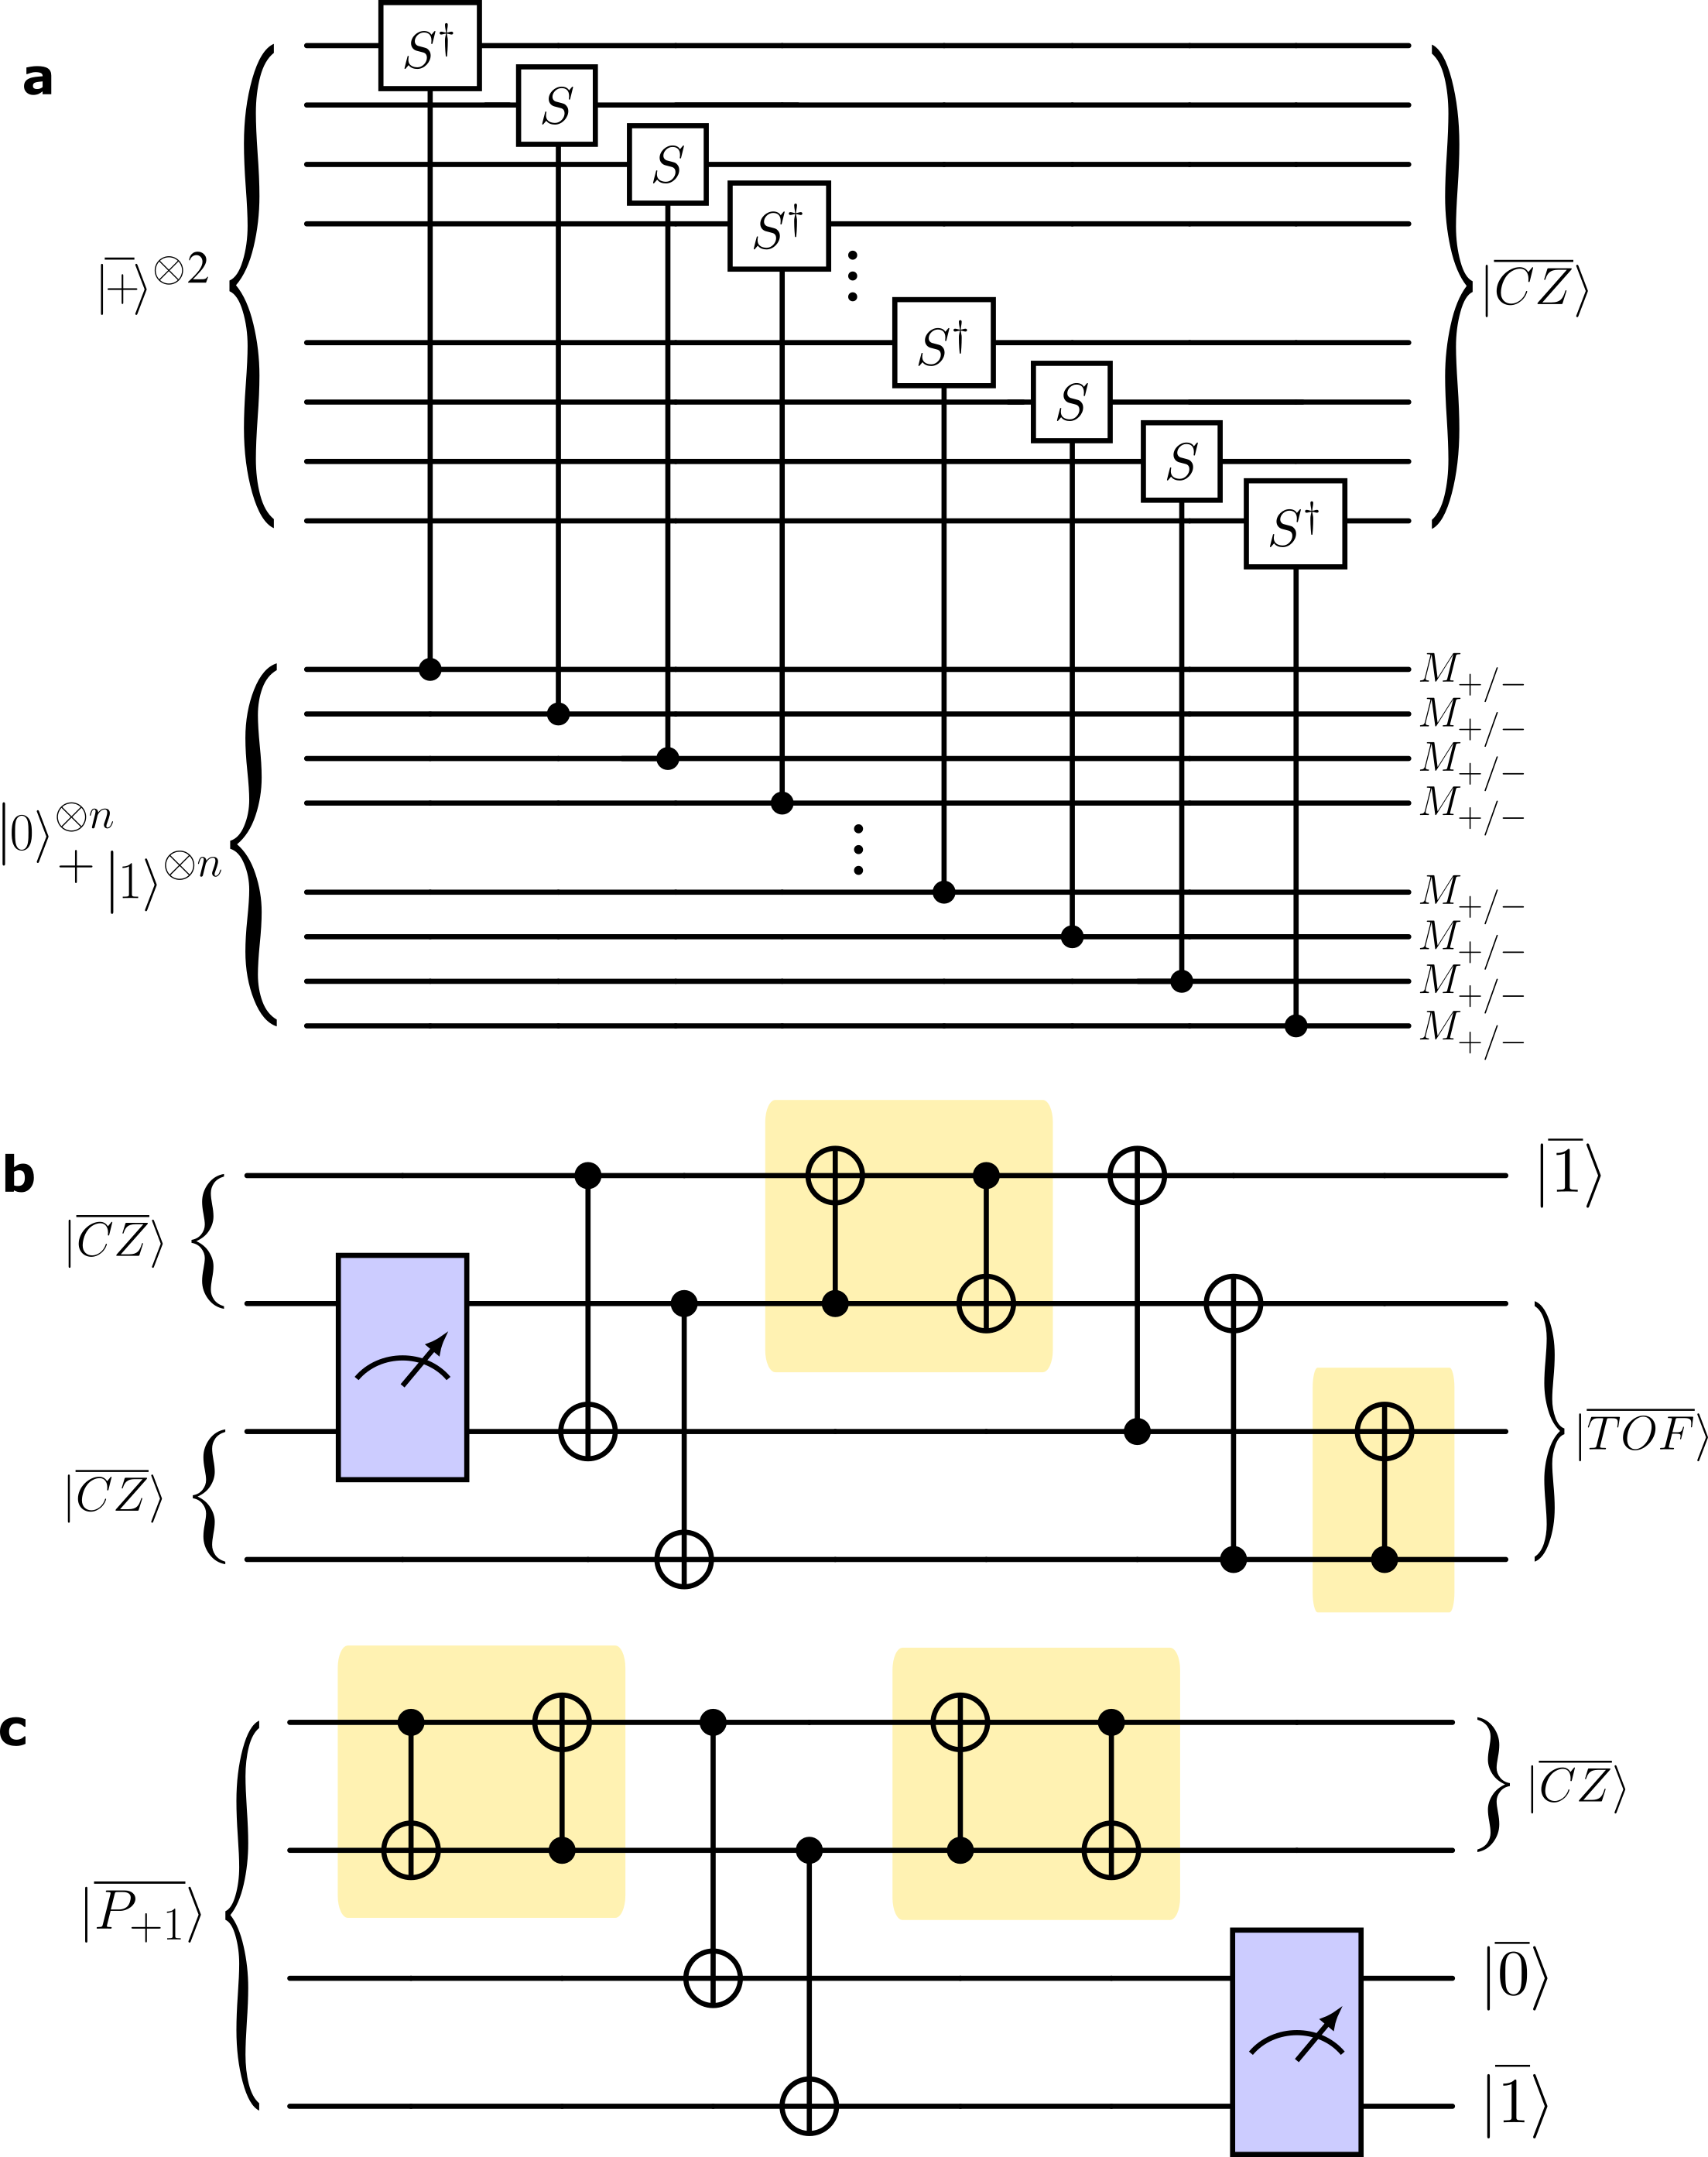
\includegraphics[width=\linewidth]{figures/cz_to_tof.png}
    \caption{\textbf{Process for distilling a $\ket{\rm TOF}$ state on the $C_4$-Helix code. a.} Circuit to zero-level distill the $\ket{CZ}$ state using the input state $\ket{+}^{\otimes n}$. Here we have depicted the ancilla as being a large cat state, $\ket{0}^{\otimes n} + \ket{1}^{\otimes n}$; however, it may be feasible to use a flagged circuit to fault-tolerantly extract the measurement result. \textbf{b.} Circuit to take two $\ket{CZ}$ states to $\ket{1}\ket{\rm TOF}$ using a $Z_2Z_3$ measurement, postselecting on the -1 outcome, and applying transversal interblock CNOT gates and SWAP-transversal intrablock CNOT gates. The circuit is immediately fault-tolerant (with inserted error correction) except for the $Z_2Z_3$ measurement. This can be made fault-tolerant with the appropriate ancillas and flags. \textbf{c.} Circuit to take the projected +1 measurement result to one that recovers one of the two input $\ket{CZ}$ states using transversal interblock CNOT gates and SWAP-transversal intrablock CNOT gates. The $Z_3Z_4$ measurement is conditioned on obtaining a -1 measurement outcome.}
    \label{fig:cz_to_tof}
\end{figure}

Following Ref.~\cite{Gupta2024}, we can use two $\ket{CZ}$ states to create a Toffoli state,
\begin{equation}
    \ket{\rm TOF} \propto  \ket{000} + \ket{010} + \ket{100} + \ket{111}
    \label{eq:toff}
\end{equation}

The procedure to do so is shown in Fig.~\ref{fig:cz_to_tof}. 
We first measure the operator $Z_2Z_3$ on $\ket{CZ}^{\otimes 2}$, which has the following action on the input state
\begin{equation}
    Z_2Z_3\ket{CZ}^{\otimes 2} \propto \sum_{\text{9 terms}}(-1)^{b+c}\ket{abcd}
    \label{z2z3}
\end{equation}
The +1 subspace is spanned by the five terms with eigenvalue +1
\begin{align}
    \ket{P_{+1}} &\propto \ket{0000} + \ket{0001} + \ket{0110} + \ket{1000} + \ket{1001},
\end{align}
while the -1 subspace is spanned by the remaining four terms with eigenvalue -1,
\begin{align}
    \ket{P_{-1}} &\propto \ket{0010} + \ket{0100} + \ket{0101} + \ket{1010}.
\end{align}


After the $Z_2Z_3$ measurement, the states $\ket{P_{+1}}$ and $\ket{P_{-1}}$ are obtained with probability 5/9 and 4/9, respectively. In the result of a -1 measurement outcome, the resulting state $\ket{P_{-1}}$ is in a convenient form to obtain the $\ket{\rm TOF}$ state, Eq.~\eqref{eq:toff}. By applying the remaining fault-tolerant circuit in Fig.~\ref{fig:cz_to_tof}(b) consisting of only transversal CNOT gates between $[[20,2,6]]$ codeblocks and automorphism gates within a codeblock, we obtain the state $\ket{1}\ket{\rm TOF}$. In the event of a +1 measurement result, we project into the $\ket{P_{+1}}$ state, which is not of a usable form; however, we can apply the circuit depicted in Fig.~\ref{fig:cz_to_tof}(c), again consisting of only transversal CNOT gates and automorphism gates, to attempt to recover one of the input $\ket{CZ}$ states. The state after the CNOT gates in Fig.~\ref{fig:cz_to_tof}(c) is 
\begin{equation}
    R_{\rm CNOT}\ket{P_{+1}} \propto \ket{0000} + \ket{1000} + \ket{0001} + \ket{1001} + \ket{0101}.
    \label{eq:pre_recovery}
\end{equation}
On this state we then measure the $Z_3Z_4$ operator. Similar to Eq.~\eqref{z2z3}, we have
\begin{equation}
    Z_3Z_4 R_{\rm CNOT}\ket{P_{+1}} \propto \sum_{\text{5 terms}} (-1)^{c+d} \ket{abcd}
\end{equation}
It can be seen that the -1 subspace is spanned by the three terms in which have the form $\ket{ab01}$. This measurement result occurs with probability 3/5, and the resulting state is $\ket{CZ}\ket{01}$. Hence we have recovered one of the two input $\ket{CZ}$ states with which we can attempt another Toffoli conversion.

Now let us estimate the resources required to successfully prepare a Toffoli state. In particular, let us estimate the number of $\ket{CZ}$ state preparation attempts (via Fig.~\ref{fig:cz_to_tof}(a)) that are needed to yield one successfully prepared Toffoli state. For simplicity, let us first assume that the input $\ket{CZ}$ states can be prepared deterministically. We then have the following costs:
\begin{itemize}
    \item Round 1: We always require 2 inputs.
    \item Retry rounds: A retry is needed with probability 5/9.
    \begin{itemize}
        \item Recover a $\ket{CZ}$ state: We recover a single $\ket{CZ}$ state from  Eq.~\eqref{eq:pre_recovery} with probability 3/5.
        \item Recover nothing: We have to create two new $\ket{CZ}$ states with probability 2/5.
    \end{itemize}
\end{itemize}

The number of times we expect to have to repeat the $Z_2Z_3$ measurement is independent of the success probability of preparing a $\ket{CZ}$ state. We project into the $\ket{P_{-1}}$ state with probability 4/9, so we expect to have to do this 1/(4/9) = 9/4 times. Hence the expected number of \textit{retries} is $E_r$ = 9/4 - 1 = 5/4. The expected cost per retry depends on the success probability of recovering a $\ket{CZ}$ state from $\ket{P_{+1}}$. Given a retry, there is a 3/5 probability we only need one additional new input $\ket{CZ}$ state, and there is a 2/5 probability we need two new input states. Hence each retry after the initial round has an expected cost of $E_c = 7/5$. The total expected inputs (assuming deterministic preparation) is then
\begin{align}
    E_s &= (\text{Cost of Round 1)} + E_r \times E_c \nonumber \\ 
        &= 2 + \frac{5}{4} \times \frac{7}{5} = \frac{15}{4}.
        \label{eq:expected_cost}
\end{align}
And so if the input $\ket{CZ}$ states could be prepared deterministically, we would expect to need 15/4 = 3.75 input $\ket{CZ}$ states on average to successfully prepare a single $\ket{\rm TOF}$ state. Let us now incorporate the fact that the probability of successfully preparing a $\ket{CZ}$ state is less than one (3/4 for the instance where the state being measured is $\ket{++}$). We can just take the expected cost of Eq.~\eqref{eq:expected_cost} and multiply by the cost per successful $\ket{CZ}$ preparation. If a $\ket{CZ}$ state is prepared with probability $p$, then the expected cost is $1/p$, and so the final cost is simply $E_C = 15/(4p)$. At $p=3/4$, this works out to needing, on average, five $\ket{CZ}$ preparation attempts per successful $\ket{\rm TOF}$ state creation. Note that this does not mean we need five $[[20,2,6]]$ codeblocks. We can reuse the codeblocks in instances where the distillation fails, so we still only need two codeblocks. Of course, the retries could be sped up if additional $\ket{CZ}$ states were already on hand. This result also indicates that there is not much benefit to switching from $\ket{++}$ to $\ket{CZ}$ for the zero-level distillation step; we only save, on average, 1.25 input $\ket{CZ}$ states at the cost of requiring an expensive arbitrary state encoder circuit.

\section{Details of the $[[60,2,12]]$ and $[[100,2,18]]$ codes}
\label{apx:big_$C_4$-Helix}

\begin{figure*}
    \centering
    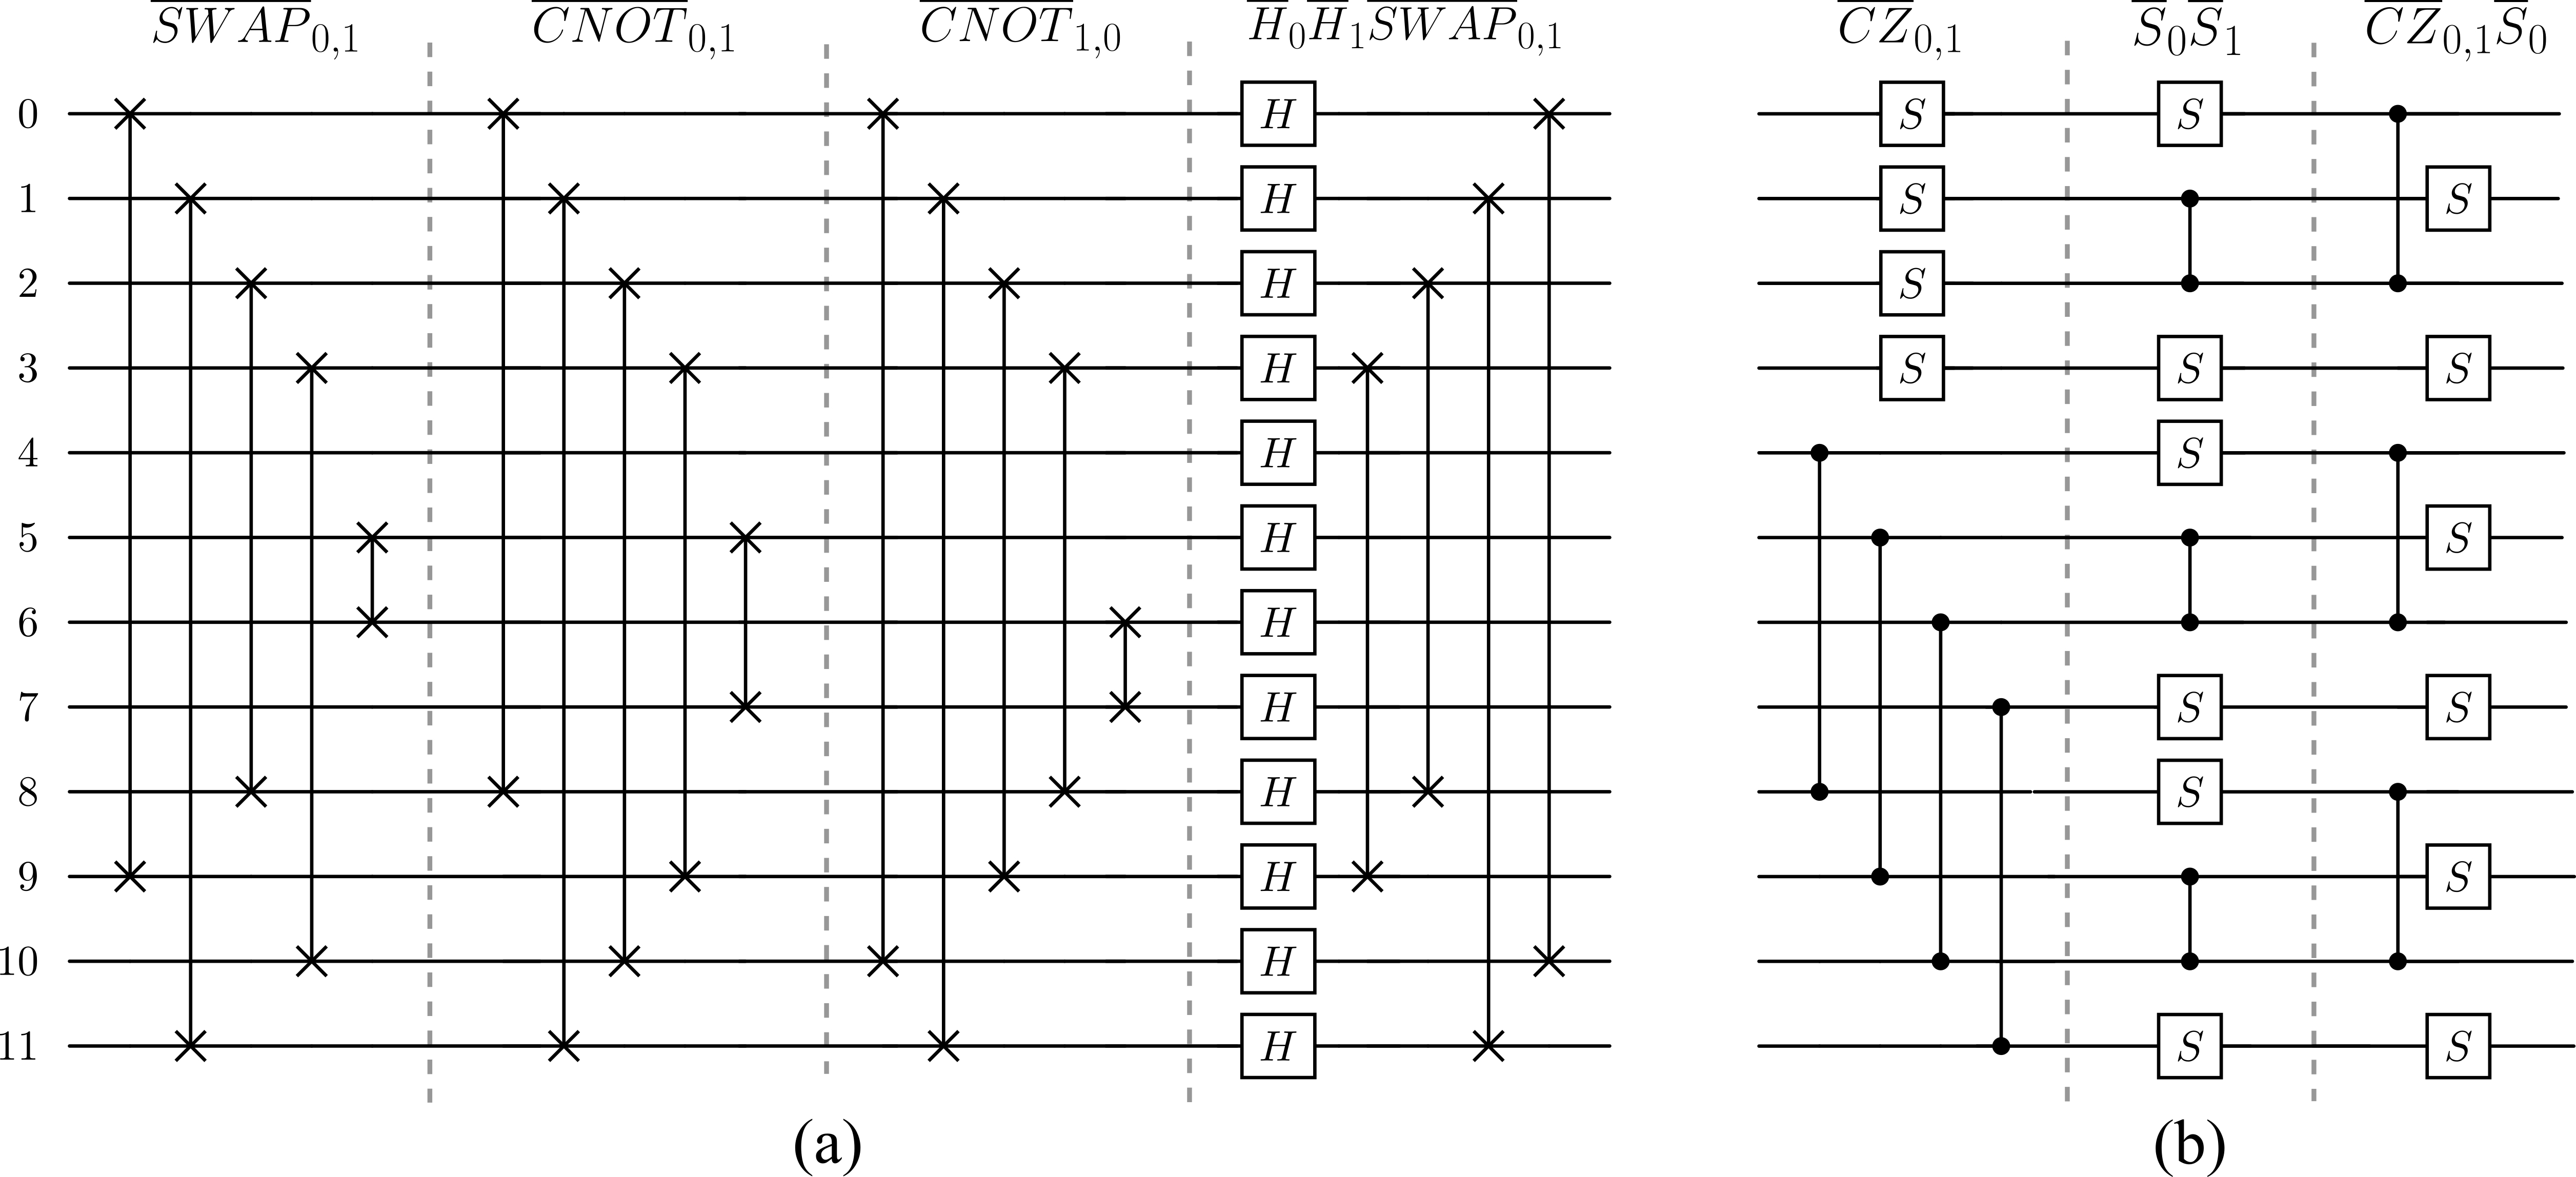
\includegraphics[width=0.9\linewidth]{figures/carbon_gates.png}
    \caption{\textbf{Logical operators for the $[[12,2,4]]$ Carbon code. a.} SWAP-transversal gates implementable using only single qubit gates and qubit relabeling. \textbf{b.} Depth-1 fold transversal gates. Note that as compared to the $[[4,2,2]]$ code, the operator $\overline{CZ}_{0,1}$ is no longer SWAP-transversal.}
    \label{fig:carbon_gates}
\end{figure*}

In this Appendix, we provide the details for larger versions of the $[[20,2,6]]$ $C_4$-Helix code, namely the $[[60,2,12]]$ \textit{Carbon-Helix} code and $[[100,2,18]]$ \textit{Double-Helix} code. As with the $C_4$-Helix code,  Appendix~\ref{apx:code_construction}, we proceed through the CSD construction until we have obtained the $[[10,2,3]]$ twisted toric code. Then, instead of concatenating along the ZX-duality $\tau: \{i,i+5\}_{0,...,9}$ with the $[[4,2,2]]$ code, we use a code with a larger distance. Using the $[[12,2,4]]$ Carbon code~\cite{paetznick2024}, the stabilizer generators and logical operators of which are given in Table IV of Ref.~\cite{paetznick2024}, yields the $[[60,2,12]]$ Carbon-Helix code. Using the $[[20,2,6]]$ $C_4$-Helix code as the lower code yields the $[[100,2,18]]$ Double-Helix code.

These code parameters are already quite competitive: the $[[60,2,12]]$ code is $4\times$ more efficient than the $[[144,1,12]]$ rotated surface code and only $2.5\times$ worse than the $[[144,12,12]]$ gross code~\cite{bravyi2023highthreshold}. Similarly, the $[[100,2,18]]$ code is $6\times$ more efficient than the $[[324,1,18]]$ rotated surface code and uses only $2\times$ more qubits than the $[[288,12,18]]$ two-gross~\cite{yoder2025} code. The benefit with this construction over these higher-rate codes is that logical computation remain simple. 

Recall that implementing logical gates on the $C_4$-Helix family can be thought of performing the logical gates of the $[[10,2,3]]$ twisted toric code on the logical qubits of the lower-level ($[[4,2,2]], [[12,2,4]], [[20,2,6]]$) codes. Thus for computation to be convenient, the required `physical' gates listed in the third column of Table~\ref{fig:actions}, $\overline{SWAP}_{i,i+5}, \overline{CNOT}_{i,i+5}$, etc., as well as in Fig.~\ref{fig:ft_phase_gate}(a), $\overline{CZ}_{i, i+5} \overline{S}_i, \overline{S}_i \overline{S}_{i+5}$, etc., must be easy to implement on the lower-level code. The $[[4,2,2]]$ code satisfies this property. Fig.~\ref{fig:carbon_gates} lists the physical circuits that implement the required logical gates on the Carbon code. The final three CZ gates of Fig.~\ref{fig:ft_phase_gate}(a) can be realized between two Carbon codeblocks with a transversal CZ gate $\{(3,2),(2,3),(8,7),(7,8),(11,10),(10,11)\}$ (unlisted indices are $i \rightarrow i$) conjugated by logical SWAPs on both codeblocks. Compared to the $[[4,2,2]]$ code, only the $\overline{CZ}_{0,1}$ gate is no longer SWAP-transversal. And so, we now have two logical gates on the Carbon-$C_4$-Helix code that require physical two-qubit gates (and hence follow-up QEC), $\overline{CZ}_{0,1}$ and $\overline{S}_0 \overline{S}_1$. Just as we did for the $C_4$-Helix code, we can build a lookup-table logical compiler that minimizes the number of QEC cycles required. The maximum number of QEC cycles needed to implement an arbitrary two-qubit logical Clifford on the Carbon-$C_4$-Helix code is four, and the full distribution is 0: 12, 1: 96, 2: 252, 3: 324, 4: 36.

Computation for the $[[100,2,18]]$ Double-Helix code follows analogously by applying combinations of $[[20,2,6]]$ gates in fifth column of Table~\ref{fig:actions} and Fig.~\ref{fig:ft_phase_gate}(c). All gates in Table~\ref{fig:actions} remain SWAP-transversal, and so we can reuse the logical compiler from the $C_4$-Helix code that minimizes the number of $\overline{S}_0 \overline{S}_1$ applications.

% With computation solved, ... Other aspects to optimize include efficient syndrome extraction circuits. One might be concerned with the high stabilizer weights of the Carbon-$C_4$-Helix (16) and $C_4$-Helix-$C_4$-Helix (24) codes; however, we can again apply adaptive syndrome extraction~\cite{Berthusen_2025} to reduce the average space-time cost of a QEC cycle. ... as the lower-level code can now correct errors. In particular, we expect to encounter an uncorrectable error with probability $p^2$ and $p^3$, respectively, and so we can refrain 




\section{Simulations}
\label{apx:simulations}

Throughout the paper, we perform circuit-level simulations with Stim~\cite{Gidney_2021} as well as Guppy~\cite{koch2025} and Selene~\cite{selene_2025}. We primarily use Guppy and Selene to estimate error rates for the Quantinuum Helios trapped-ion quantum processor, and we use Stim to probe the low error-rate regime. We use the following circuit-level noise model:
\begin{itemize}
    \item Qubit reset operations have a probability $p$ of preparing the $\ket{1}$ state instead of the $\ket{0}$ state.
    \item Qubit measurement operations have probability $p$ of yielding a flipped result.
    \item The single-qubit depolarizing channel is applied after single-qubit gates with probability $p/10$.
    \item The two-qubit depolarizing channel is applied after two-qubit gates with probability $p$.
    \item The single-qubit dephasing (Z) channel is applied during idle operations with probability $p/10$.
\end{itemize}
Note that when simulating Helios, we instead adopt a device-specific stochastic Pauli error model derived from  benchmarking data~\cite{Ransford2026}.

\subsection{Defining Detectors and Sign Tracking}
We perform circuit-level decoding over the entire circuit with a detector error model (DEM) generated from Stim. In a standard memory experiment, rows of this matrix, referred to as detectors, are formed from parities of time-adjacent syndromes, $D_i^{(t)} = \sigma_i^{(t)} \oplus \sigma_i^{(t-1)}$, where $\sigma_i^{(t)}$ denotes the $i^{\rm th}$ syndrome measured at time $t$. In particular, since we prepare the logical state by projectively measuring the $Z$-type stabilizer generators (after initializing all physical qubits in the $\ket{+}$ state), the $Z$-syndromes will be initialized with random signs and it is necessary to make detectors out of parity difference rather than individual syndromes. Defining the detectors from the parity of time-adjacent syndromes (instead of the parity with respect to the random sign at initialization) would further help with localizing errors in space-time and thus can help with the decoding speed and accuracy. Here we are using space-time local loosely to mean local with respect to the graph representation of the circuit, since the checks for the $C_4$-Helix codes are geometrically non-local. In the presence of logical gates, such as in randomized logical Clifford benchmarking, building the detectors is more involved since one needs to track the random syndrome signs as they propagate from one stabilizer to another. While logical gates preserve the original codespace where all standard stabilizer generators have $+1$ sign, they do not necessarily preserve the image codespaces defined by random signs of the stabilizer generators resulting from projective state prep; Instead, the logical gates result in a deterministic linear mapping between the signs of the stabilizers before and after the logical gate. As such, $\sigma_i^{(t)}$ and $\sigma_i^{(t-1)}$ may no longer be related after applying some logical gate $\overline{U}$ at time $t$. We can determine how the current syndromes relate to the previous syndromes by using the transformation matrix $T$ that relates the stabilizer generators before and after the application of the logical gate.
\begin{equation}
    \mathcal{S} \mapsto \mathcal{S}'=T\mathcal{S}.
    \label{eq:stabs}
\end{equation}
Here, $\mathcal{S}$ is the  $\mathbb{F}_2^{(n-k) \times 2n}$ symplectic matrix describing the stabilizer generators of the code and $\mathcal{S}'$ is  their image in symplectic form under the logical gate $U$ and $T$ is the $\mathbb{F}_2^{(n-k) \times (n-k)}$ matrix relating them to each other. When applying multiple logical operations $\overline{U} = \overline{U}_i\overline{U_j}...\overline{U}_k$, between syndrome extraction rounds, either a total $T$ can be computed, or $T_i$'s for each $\overline{U}_i$ can be computed and composed $T = T_iT_j...T_k$. With $T$ computed, valid detectors are formed as
\begin{equation}
    D_i^{(t)} = \sigma^{(t)}_i \oplus (T^{-1}\sigma^{(t-1)})_i,
\end{equation}
since $T^{-1}\mathcal{S}$ gets mapped to $\mathcal{S}$ under $U$.
When using the image codespaces with non-trivial stabilizer signs, it is also necessary to track how the logical observables change under the application of logical gates. That is because in the presence of random stabilizer signs, logical operators which differ by a stabilizer are only equivalent up to a sign, making it necessary to track how the signs of the logical observables change as the result of the presence of random stabilizer signs as they propagate through logical gates. Just as we did for the stabilizer generators, we can keep track of the relative signs of $X$ and $Z$ logical operators $\overline{\sigma}_{X,j}^{(t)}$ and $\overline{\sigma}_{Z,j}^{(t)}$ for $j \in \{1,\cdots,k\}$ as they propagate through logical gates. We note that $\overline{\sigma}_{P,k}^{(t)}$ only tracks the relative signs that logical observables acquire under a logical Clifford gate and has nothing to do with the actual value of the logical operator. To track how $\overline{\sigma}_{P,j}^{(t)}\in \mathbb{F}_2^{2k}$ changes under a logical operation, we compute the action of the physical gate sequence on the symplectic representation of the $X$ and $Z$ logical operators: 
\begin{equation}\label{eq:ULTS}
    \mathcal{L}\mapsto \mathcal{L}^* = U \mathcal{L} \oplus T' \mathcal{S}.
\end{equation}
Here $T' \in \mathbb{F}_2^{2k \times (n-k)}$ represents the contribution from the stabilizer generators and $U\in \mathbb{F}_2^{2k \times 2k}$ represents the logical action of the Clifford gate $U$ in the symplectic form. Accordingly, the relative signs of the logical operators can be tracked as:
\begin{equation}
    \overline{\sigma}_{P,k}^{(t)} = (U^{-1}\overline{\sigma}^{(t-1)})_{P,k} \oplus (U^{-1} T' T^{-1}\sigma^{(t-1)})_{P,k}.
\end{equation}
This is because it follows from Eqs.~\eqref{eq:ULTS} and \eqref{eq:stabs} that $U^{-1}\mathcal{L}\oplus U^{-1} T' T^{-1}\mathcal{S}$ gets mapped to $\mathcal{L}$ under the corresponding Clifford operation. When measuring an observable at the end of the circuit, one should multiply the outcome by the relevant relative sign $\overline{\sigma}^{(t)}_{P,k}$ to cancel the sign that has been acquired due to random stabilizer signs. We set $\overline{\sigma}^{(0)}_{P,k}=+1$ at the start of the circuit.
% When $T$ is nonzero, a measurement of $\mathcal{L}^{(t-1)}$ will not be deterministic. Such is the case for certain sequences in Clifford randomized benchmarking, even though the sequence $\overline{G}_0 \overline{G}_1 ... \overline{G}^{-1}$ resolves logically to the identity. To recover a deterministic observable, certain stabilizer measurement results, those specified by $T'$, must be added to the constructed $\mathcal{L}^{(0)}$ outcome. \nb{to iteratively track you need $U^\dagger$...}
% Instead of computing an overall $T'$ for some long sequence of gates $\overline{U} = \overline{U}_i\overline{U_j}...\overline{U}_k$, it can be tracked iteratively. 
% \begin{equation}
%     \mathcal{L}^{(t)}
% \end{equation}
% inverse gate sequence ... $U^\dagger$ ... 

We remark that the sign tracking can be entirely dropped if all stabilizers are initialized in their +1 eigenspace, e.g. by a unitary preparation circuit~\cite{forlivesi2025} or by applying destabilizers to any generators with an initial measured value of -1. In that case each syndrome can be a detector by itself. Those detectors however are not local in space-time, so decoders can still benefit from sign tracking of the syndromes as it results in space-time local detectors.



\subsection{Frontier decoding and confidence-based postselection}
\label{apx:decoder}

We decode the hardware experiments using the Frontier decoder~\cite{leverrier2026}, a pruned dynamic-programming decoder that approximates logical maximum-likelihood decoding. For a detector error model, let $x$ denote a fault configuration, $H$ the detector matrix, and $L$ the corresponding logical-observable matrix, such that
\begin{equation}
    Hx=s, \qquad Lx=\ell,
\end{equation}
where $s$ is the observed detector syndrome and $\ell$ labels the resulting logical class. The probability mass associated with a logical class is
\begin{equation}
    Z_\ell(s)
    =
    \sum_{\substack{x:Hx=s\\Lx=\ell}}
    \Pr(x).
\end{equation}
Logical maximum-likelihood decoding chooses the class with the largest $Z_\ell(s)$.

Frontier approximates these logical-class masses by processing fault variables sequentially while retaining a small set of boundary states. Each boundary state records the residual syndrome on the active detector boundary together with its accumulated logical label. States with identical boundary data are merged by summing their probability masses, after which low-scoring states are pruned. At the end of the circuit, the retained states are aggregated according to logical class, giving approximate masses $\widehat{Z}_\ell(s)$, and the decoder returns
\begin{equation}
    \ell^*
    =
    \text{arg max}_\ell \widehat{Z}_\ell(s).
\end{equation}
For the hardware experiments and for the simulations below, we apply Frontier directly to the detector error model of the entire circuit volume. However, we note that, through its narrow-frontier construction, Frontier naturally supports streaming decoding, for which memory requirements and latencies need not grow with the total circuit depth. We leave it to future work to develop the streaming version and to interface it with a quantum computer.

Since even distance codes can detect higher weight errors than can be reliably corrected, it is (optionally) possible to improve their performance through post-selection on detection of high weight errors.
Forced gap decoding~\cite{gidney2023, lee2026, xie2026, wills2026} is a general post-selection technique which can potentially improve the success probability of the decoding task at the expense of a tunable post-selection rate. Given a decoder $D$, syndrome $s$, and a set of observables $(o_1,\cdots,o_k)$, let $E^*=D(s)$ be the error that the decoder $D$ finds when decoding the syndrome $s$ and let $l^*\in \mathbb{Z}_2^{k}$ be the vector that specifies which observable value is flipped by $E^*$. Let $C(E^*)$ denote the cost of $E^*$, which is a measure of how unlikely it is for this error to happen. One can quantify the decoder's confidence in its solution by looking a the difference between $C(E^*)$ and $C(\widetilde{E}^*)$ where $\widetilde{E}^*$ is the error that the decoder would have found if it was restricted to solutions for which $\widetilde{l}^*\ne l^*$. For example if $E^*$ is the most likely error, $\widetilde{E}^*$ would be the most-likely error which is not logically equivalent to $E^*$. If $C(\widetilde{E}^*) \approx C(E^*)$, the decoder is not very confident on the solution it has found, while $C(\widetilde{E}^*) \gg C(E^*)$ means that $E^*$ is a high confidence solution. Forced-gap postselection rejects shots for which this separation falls below a chosen threshold.

For decoders that return only a single preferred correction, determining $\widetilde{E}^*$ generally requires additional constrained decoding calls in which the logical outcome is forced to differ from $\ell^*$. Frontier makes this comparison directly available: because its terminal output retains probability mass resolved by logical class.
%, no additional decoding calls are required. 
We define the Frontier confidence gap as
\begin{align}
    \Gamma(s)
    &=
    \log \widehat{Z}_{\ell^*}(s)
    -
    \max_{\ell\neq\ell^*}
    \log \widehat{Z}_{\ell}(s) \\
    &=
    \log
    \frac{\widehat{Z}_{\ell^*}(s)}
    {\widehat{Z}_{\ell^{(2)}}(s)},
\end{align}
where $\ell^{(2)}$ denotes the second-most-likely logical class. Larger values of $\Gamma$ indicate greater separation between the decoder's preferred logical class and its nearest competitor. For forced-gap postselection, we choose a threshold $\gamma$ and reject a shot whenever $\Gamma(s)<\gamma$. The threshold $\gamma$ can be tuned to trade logical error rate against post-selection overhead.

\subsection{Low error-rate simulations}
%
\begin{figure}[t]
    \centering
    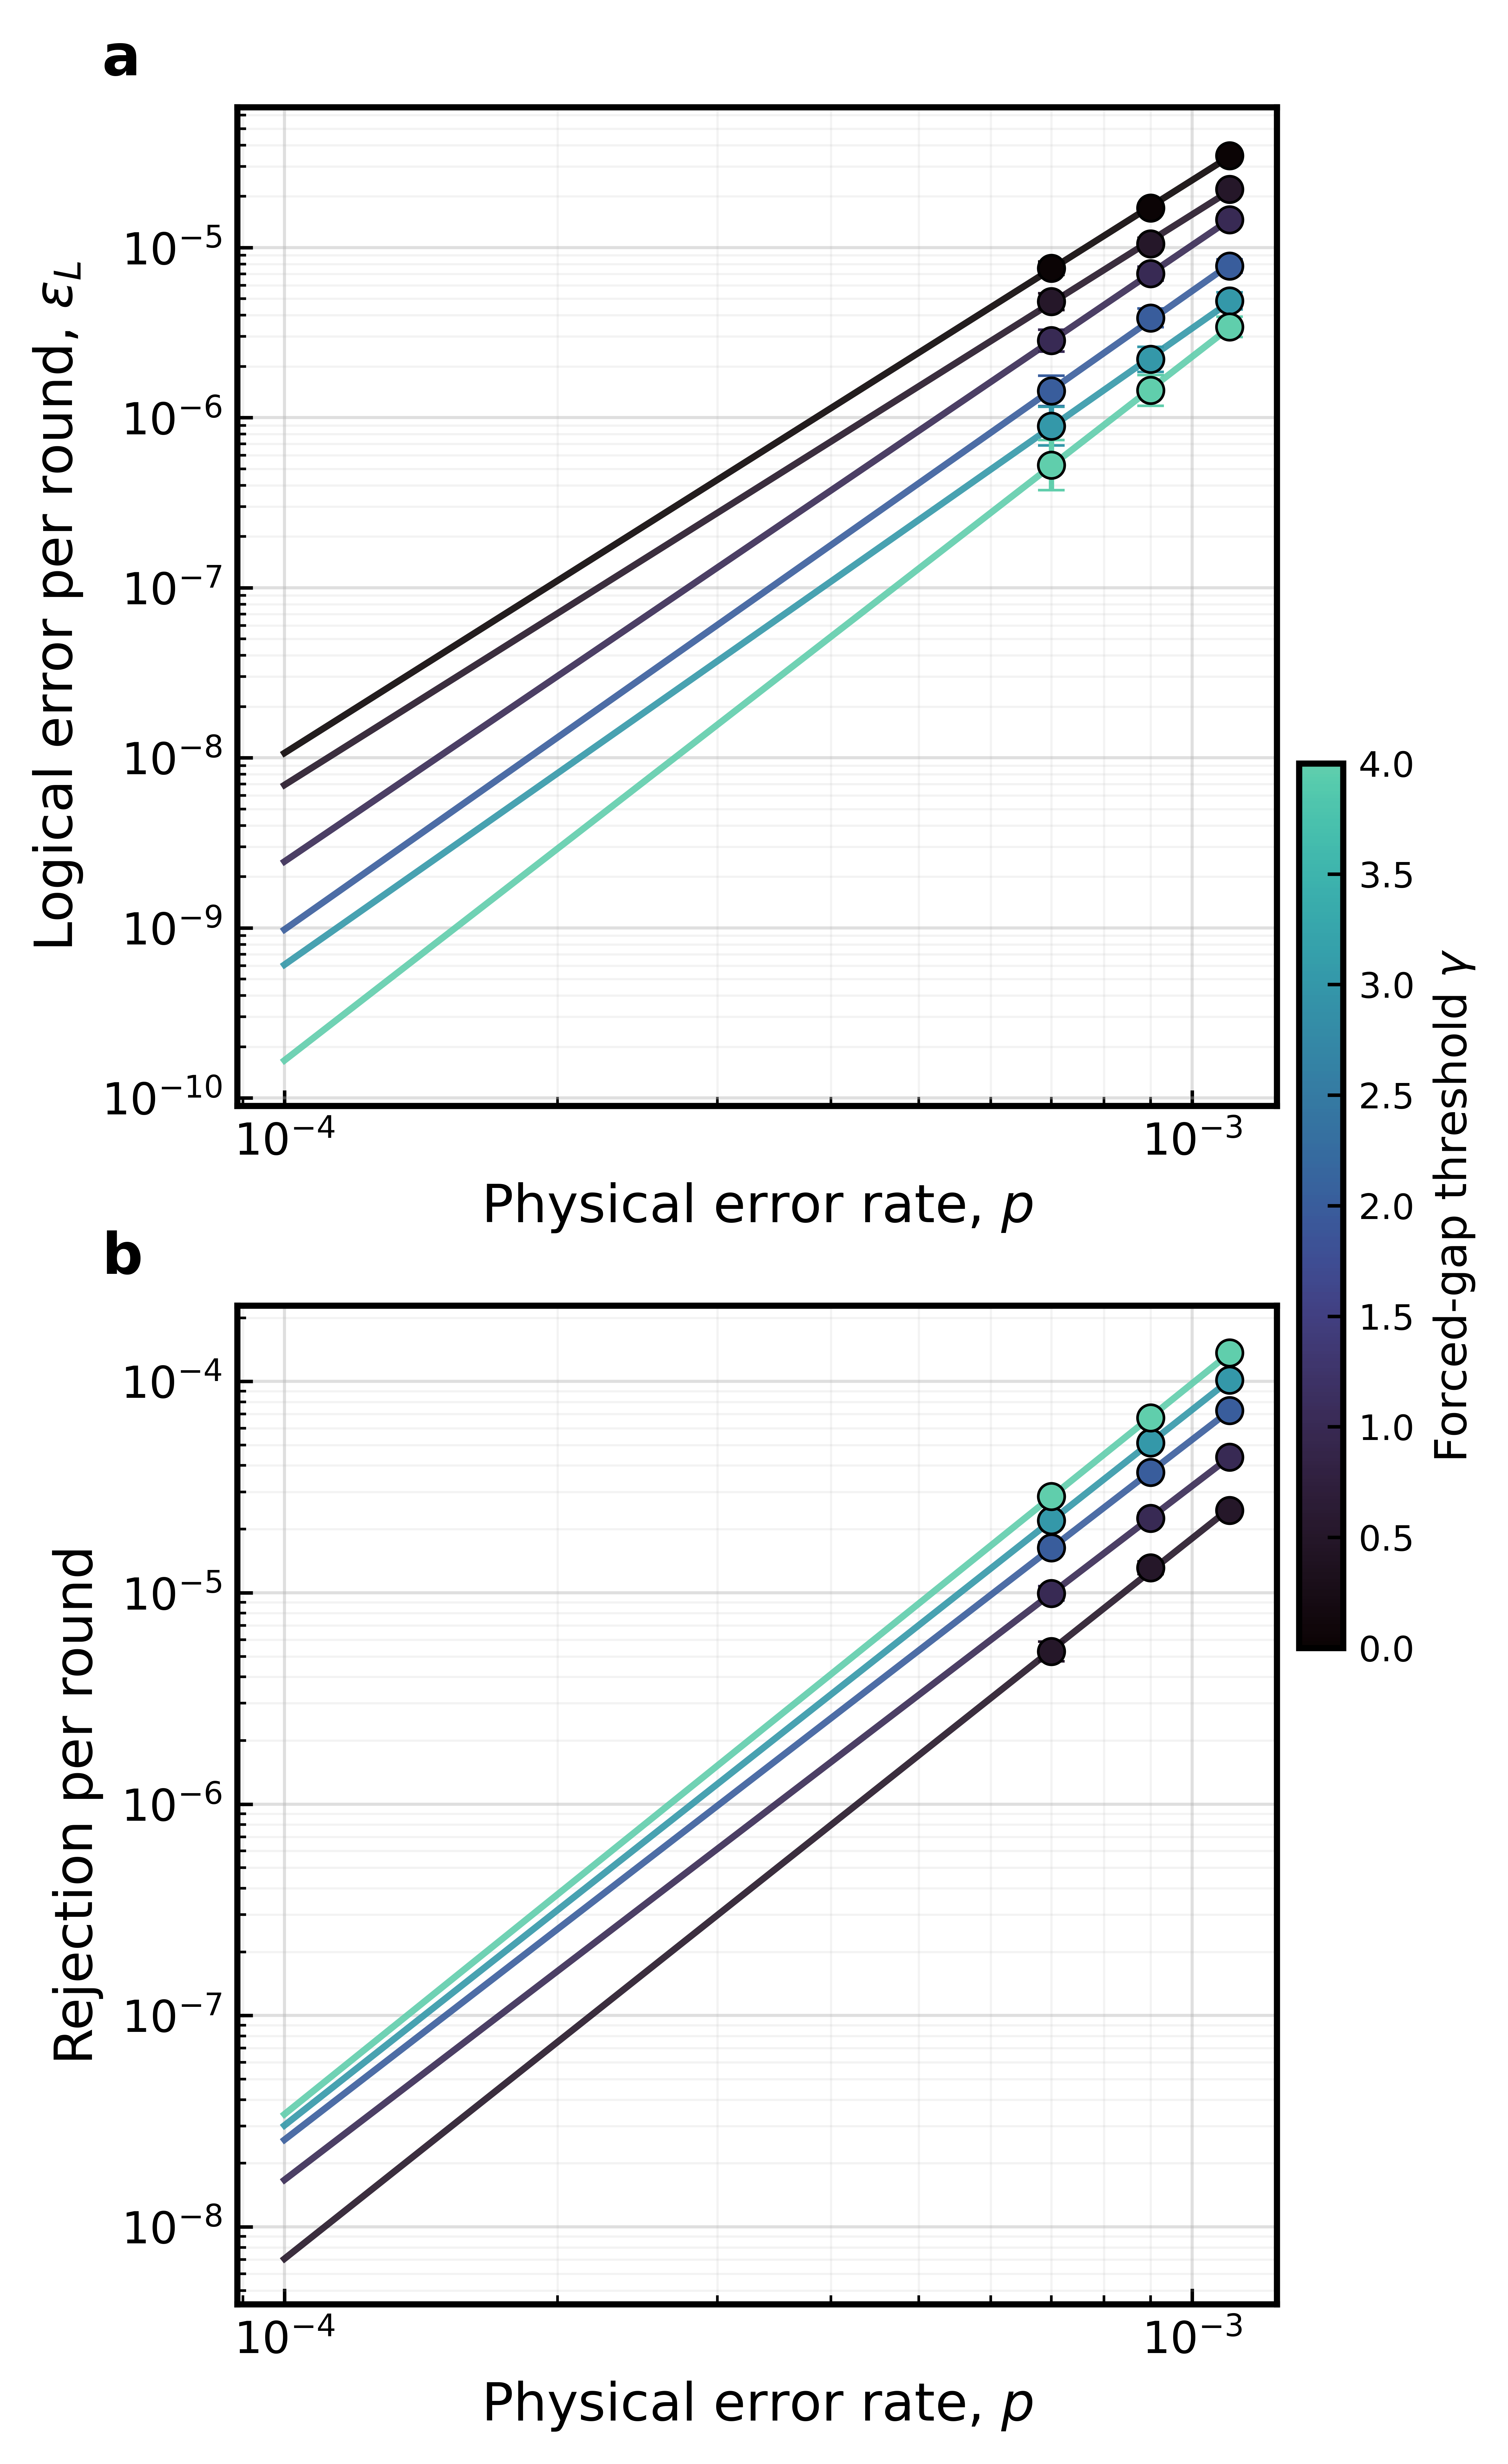
\includegraphics[width=0.95\linewidth]{figures/frontier_extrapolation_memory.png}
    \caption{\textbf{Low physical error rate memory experiment simulations.} Memory simulations of the $[[20,2,6]]$ code as prepared using projective measurement and decoded using Frontier over the entire $r=12$ rounds of syndrome extraction. \textbf{a.} Logical error rate per round as a function of the physical error rate. \textbf{b.} Postselection rate per round as a function of the physical error rate. For $\gamma=0$, no postselection is performed. Postselection intensity ($\gamma$) is indicated by the line color.}
    \label{fig:memory_frontier}
\end{figure}
%
In this section, we present additional circuit-level simulations extended to physical error rates as low as $p= 10^{-4}$--- a regime motivated by two-qubit gate infidelities already demonstrated in trapped-ion testbeds~\cite{hughes2025}. Despite the \chelix{} code only having a distance of six, we find that, when combined with modest postselection from the Frontier decoder, logical error rates per round near $10^{-10}$ are obtainable. The memory experiments follow those described in the main text: we prepare the $[[20,2,6]]$ code using projective measurements in either the $\ket{\overline{00}}$ or $\ket{\overline{++}}$ states, perform $r=12$ rounds of syndrome extraction using the syndrome extraction circuit of Section~\ref{apx:syndrome_extraction}, and then destructively measure out the data qubits in the same basis in which they were prepared. From this final destructive measurement we can construct the syndromes and logical operators of a single type. We decode using Frontier and potentially perform postselection with $\gamma \le 4$. The logical error rate per round is then obtained as $\epsilon_L = 1 - (1 - p_L(r))^{1/r}$. As opposed to the main text, in this Appendix we report block error rate as opposed to a normalized per LQ error rate. Fig.~\ref{fig:memory_frontier}(a) displays $\epsilon_L$ as a function of the physical error rate, where we have averaged over the $X$ and the $Z$ bases. We fit the data to a power law and extract exponents that match reasonably well with the expected value of $\lfloor(d-1)/2\rfloor + 1$. Fig.\ref{fig:memory_frontier}(b) shows the postselection rate per round as a function of the physical error rate for varying $\gamma$. For $\gamma > 0$, the rejection rate per round exceeds the logical error rate per round, and so a long computation will be limited by accepted shots. However, for certain applications---in particular, those in which a small number of highly accurate shots are desirable---then the reduced logical error rate may justify the associated sampling overhead.


\begin{figure}
    \centering
    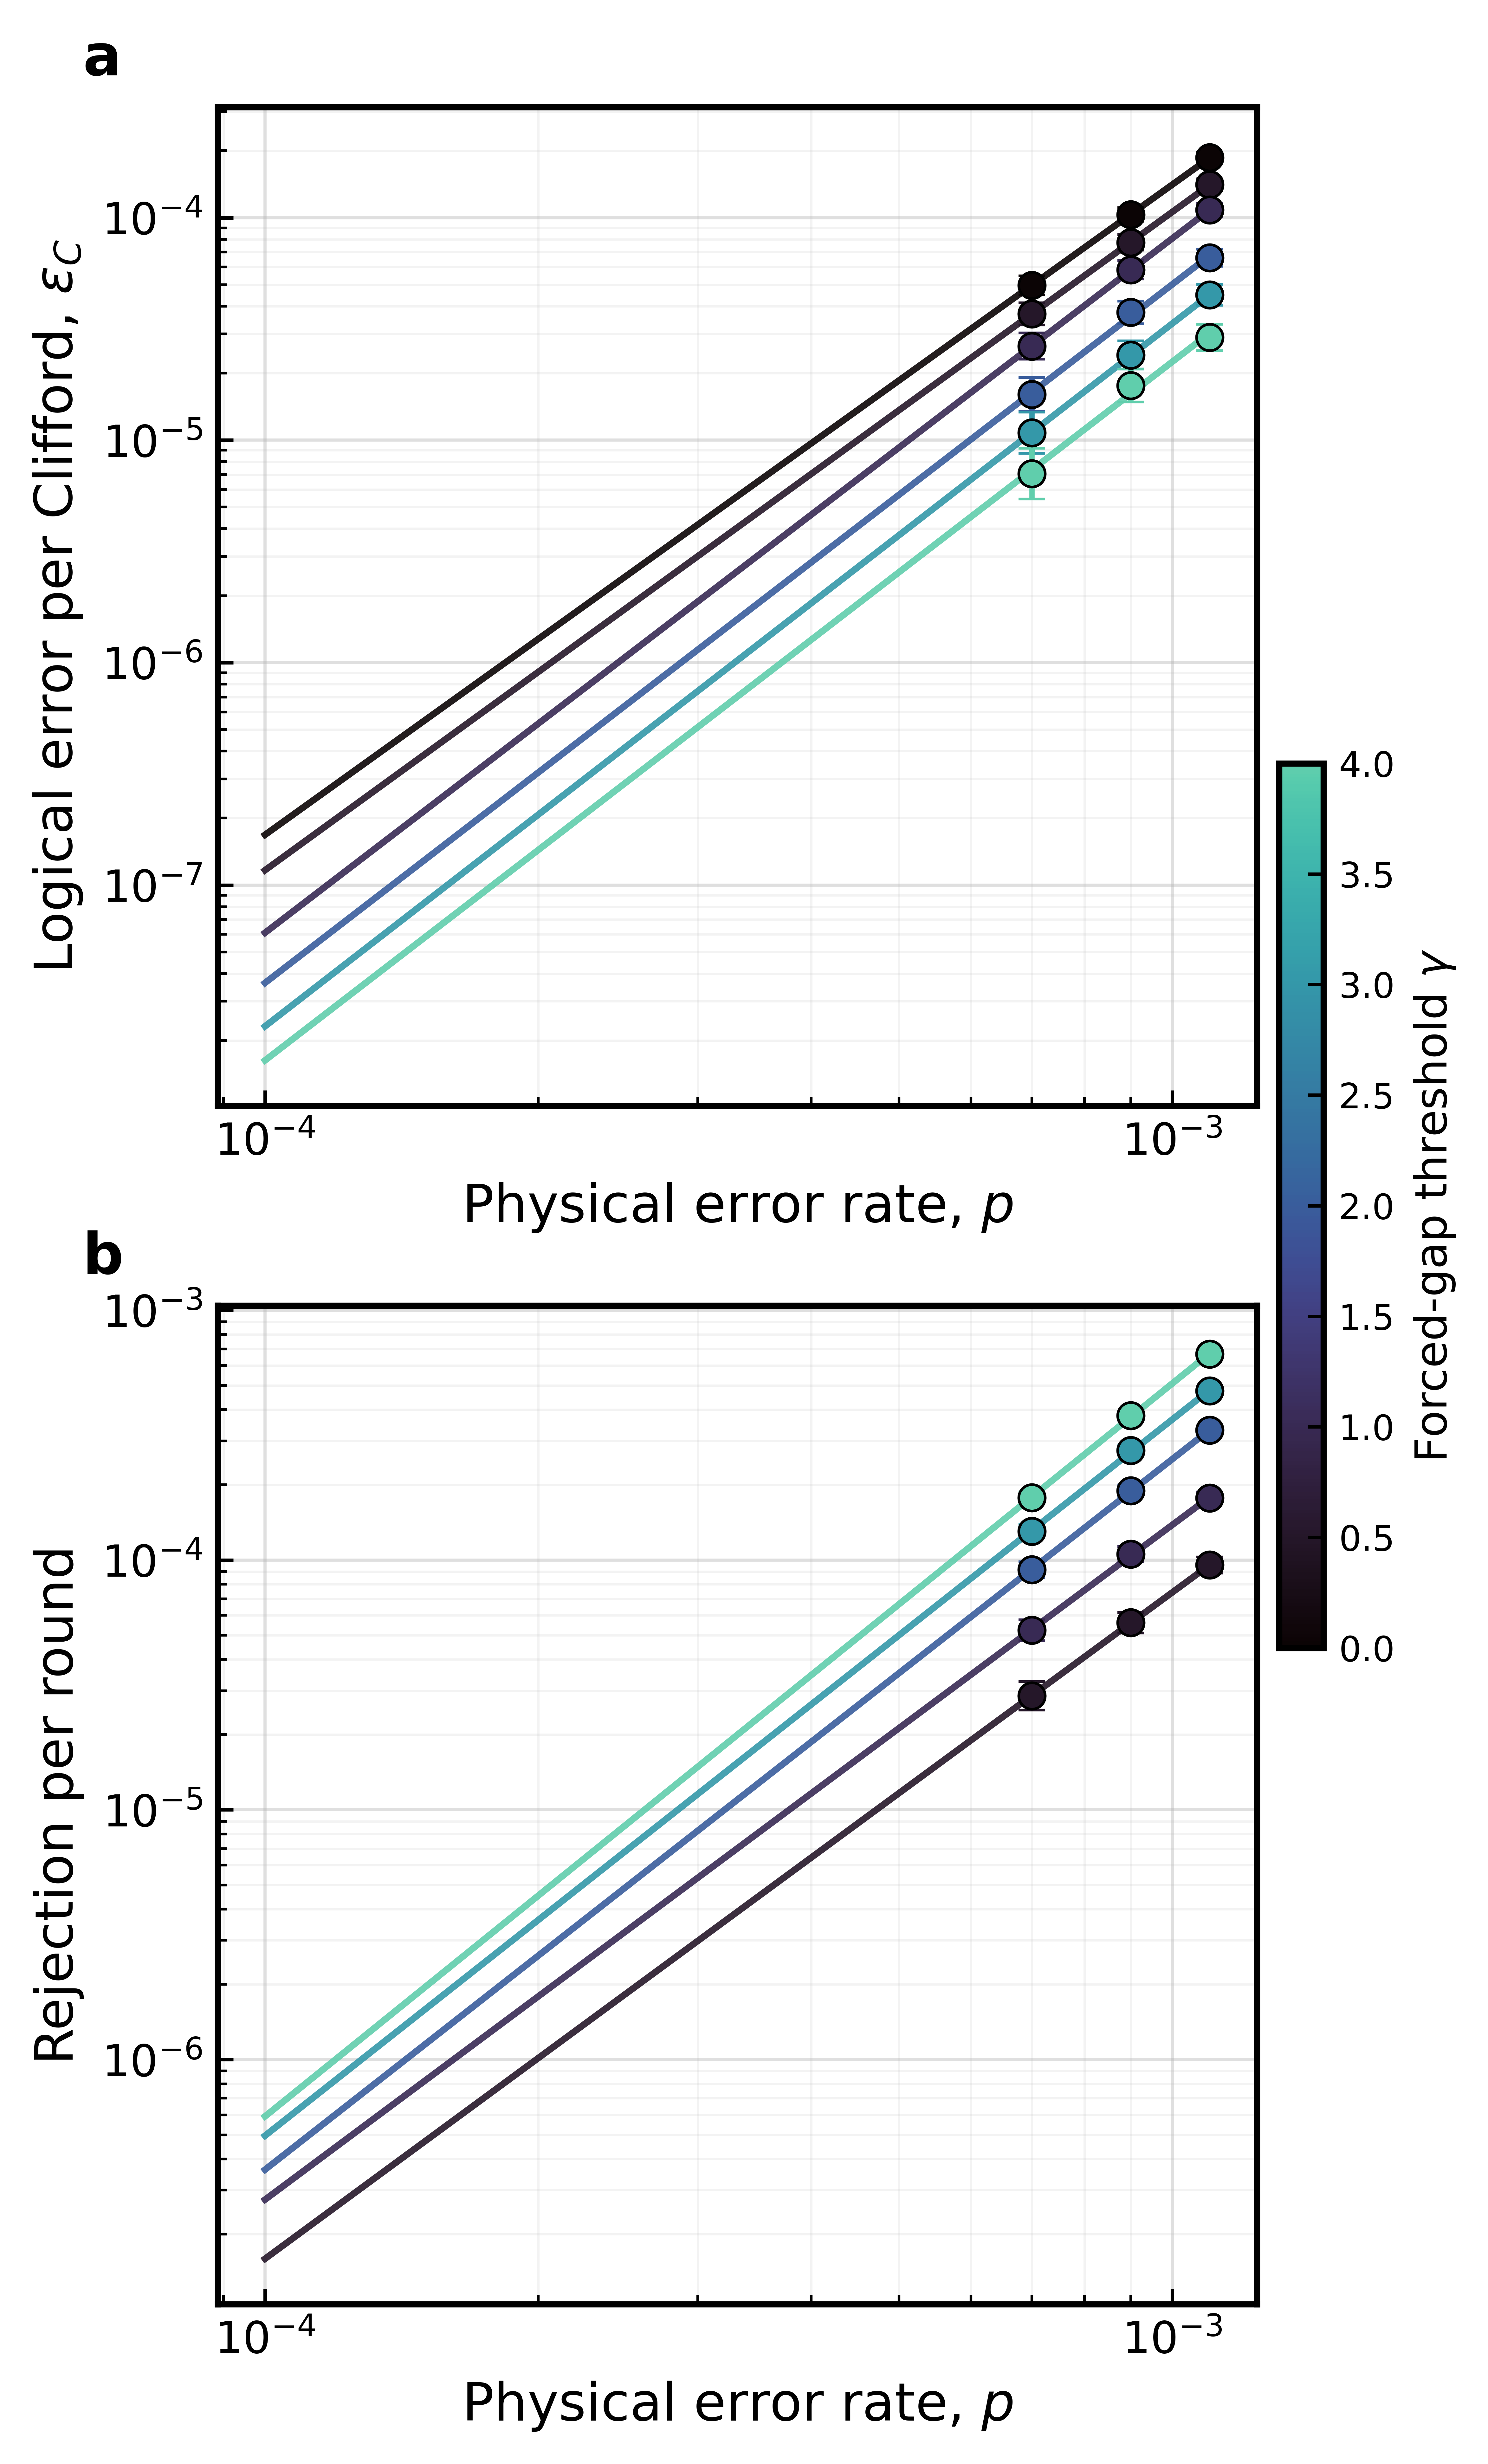
\includegraphics[width=0.95\linewidth]{figures/frontier_extrapolation_logic.png}
    \caption{\textbf{Low physical error rate intrablock logic.} TQRB simulations of the \chelix\ code decoded using Frontier over the entire $m=6$ ($r=7$) Clifford sequence. \textbf{a.} Logical error rate per Clifford as a function of the physical error rate. \textbf{b.} Rejection rate per Clifford as a function of the physical error rate.}
    \label{fig:randomized_bencharking_sims}
\end{figure}

We additionally simulate randomized Clifford benchmarking to estimate the fidelity of performing logical intrablock Clifford operators. The simulations again follow the experiment run in the main text: we perform $m$ random logical two-qubit Clifford operators acting on a single \chelix\ codeblock. Having tracked the total accumulated Clifford operator, we calculate and apply a final inverse to return the code to the initial $\ket{\overline{00}}$ state. We again decode using Frontier over the entire circuit volume and optionally apply forced-gap postselection. The logical error rate per Clifford is calculated as above, but with $r = m+1$ `rounds' of logical gates. Fig.~\ref{fig:randomized_bencharking_sims}(a) reports the obtained logical error rates when extrapolated down to physical error rate $10^{-4}$. We see higher error rates for logic than for memory experiments which is expected due to a number of factors: each random Clifford contains on average 1.5 syndrome extraction rounds, the $\overline{S}_0 \overline{S}_1$ gate incorporates (flagged) in-block physical CZ gates which nonetheless present opportunities for errors to accumulate, and the decoding problem is more complex. We note that random intrablock Clifford operators are a worst-case workload for the \chelix\ code. In practice, clever physical-to-logical assignment can make it so most if not all intrablock Cliffords are automorphisms or transversal operations~\cite{LeBlond2026InPrep}. 

\begin{figure}
    \centering
    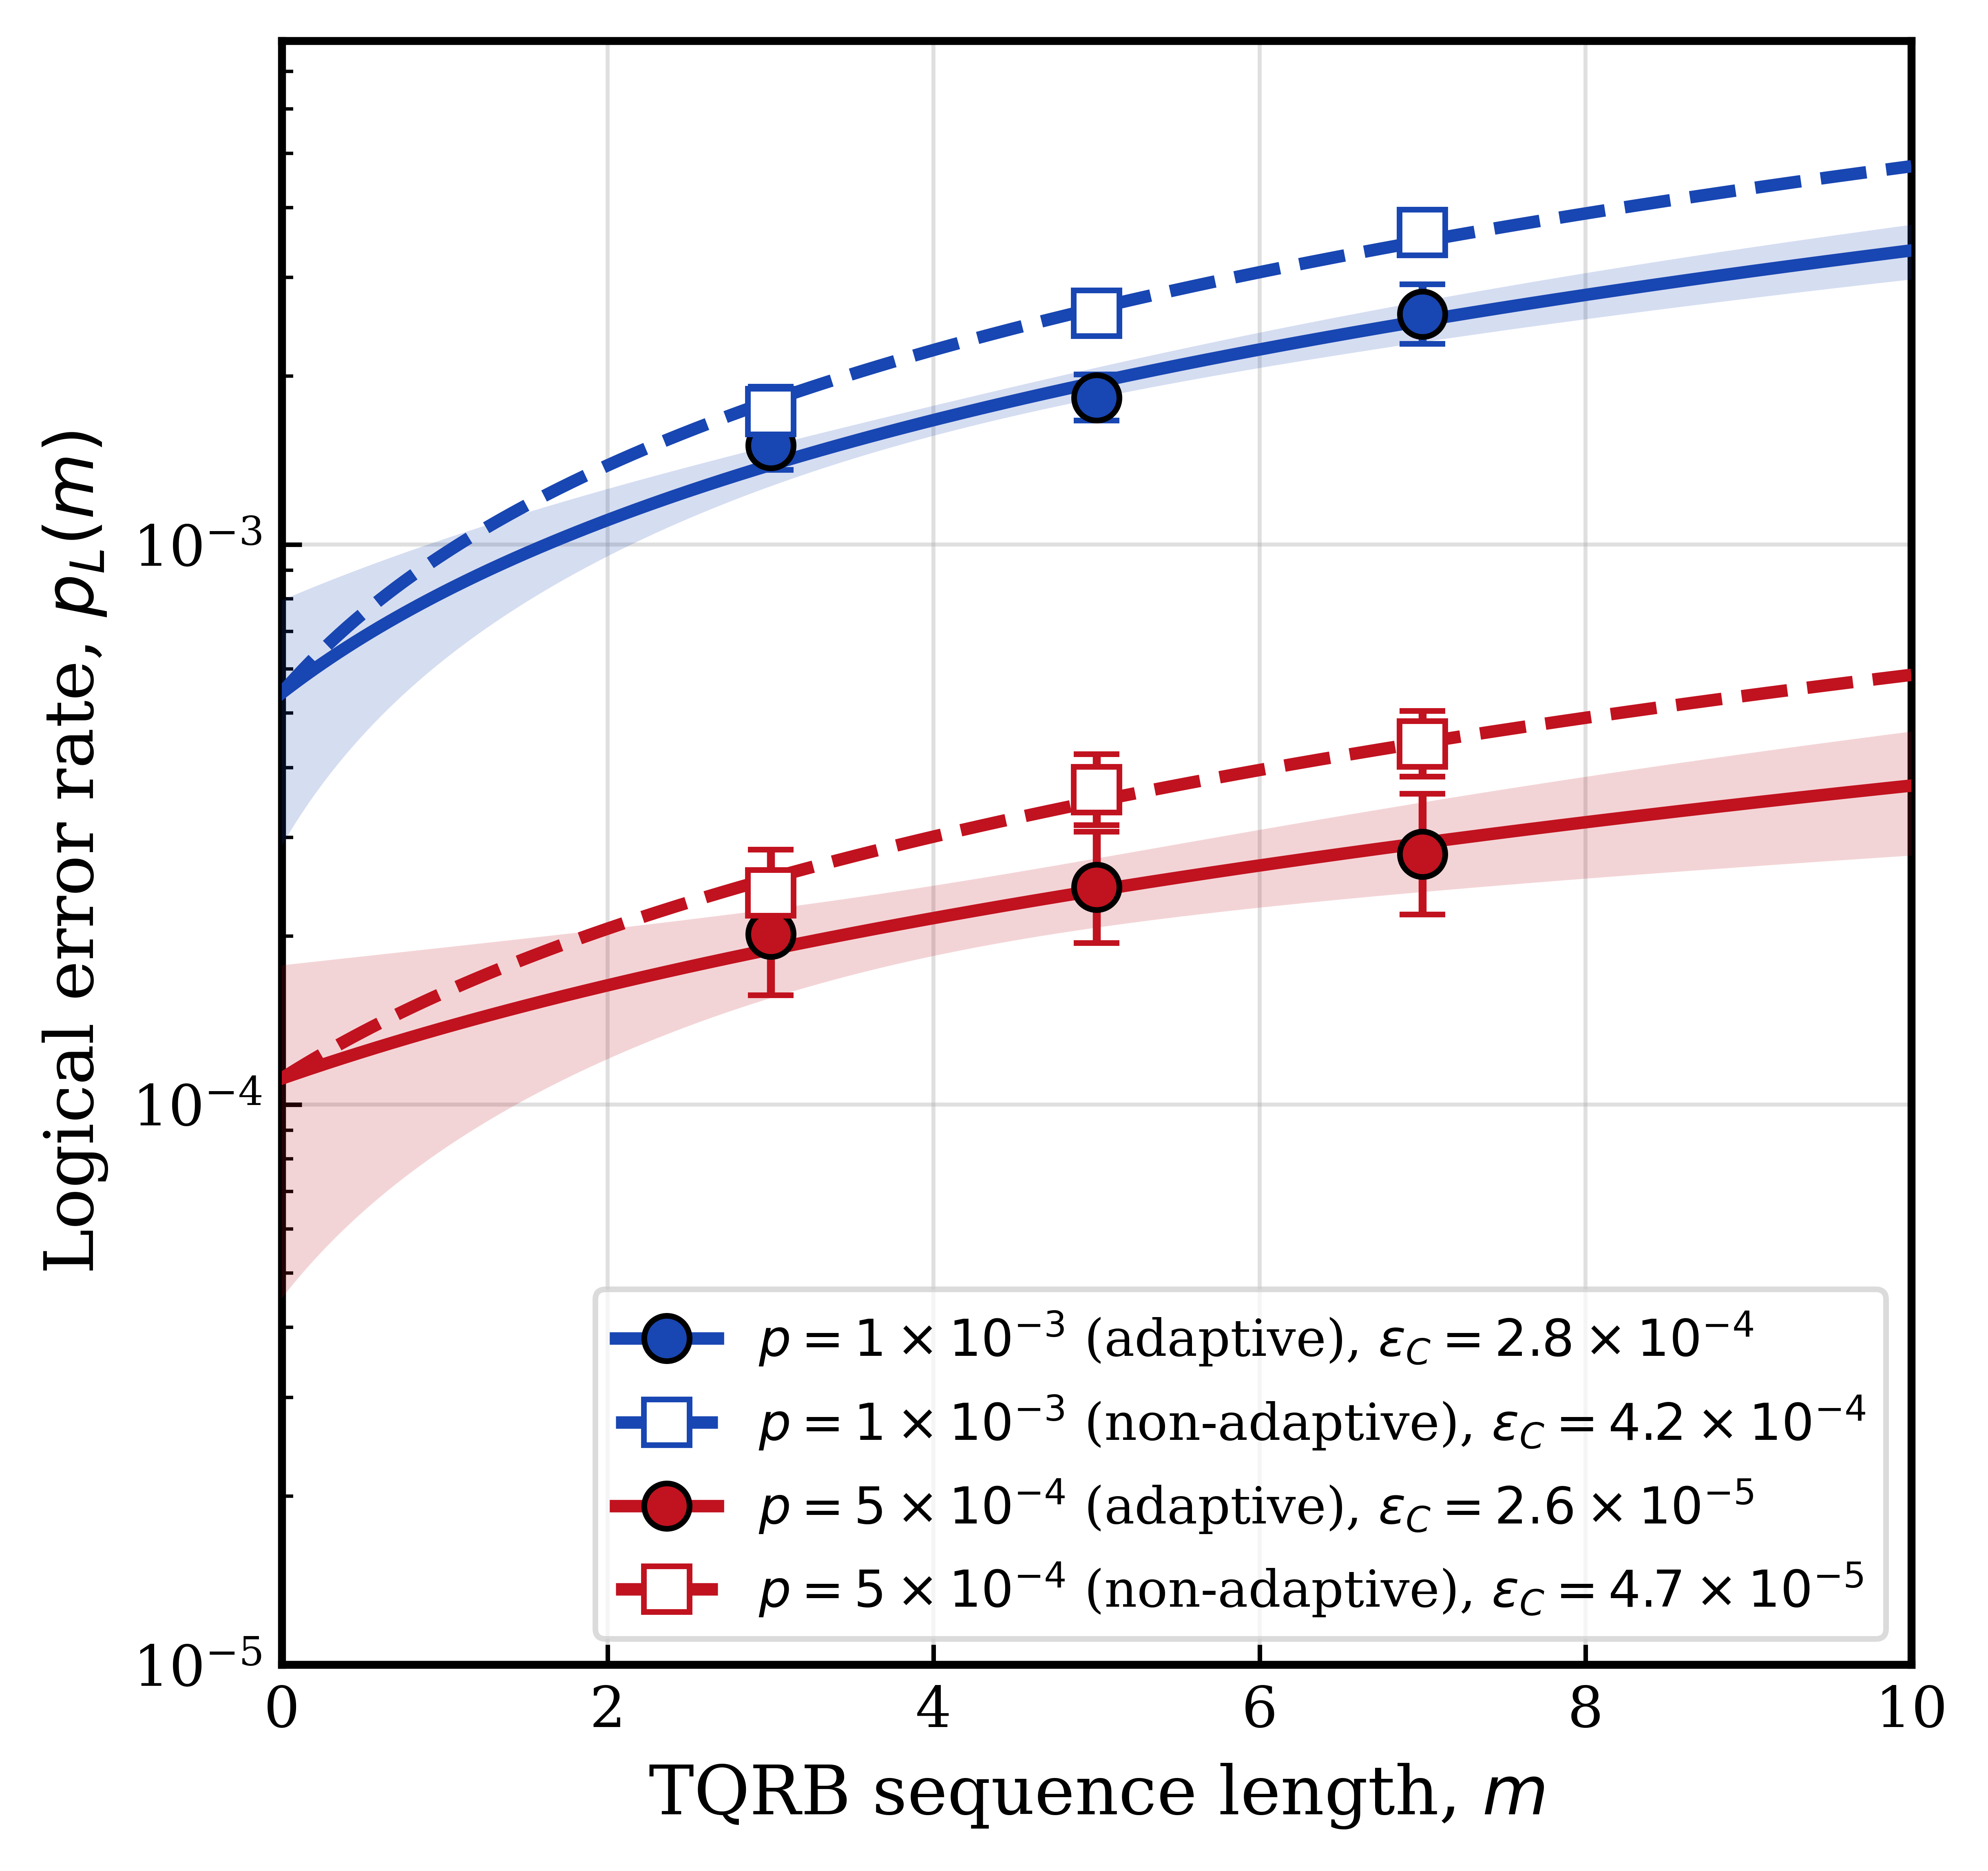
\includegraphics[width=0.9\linewidth]{figures/logic_sims.png}
    \caption{\textbf{Comparison of adaptive and nonadaptive syndrome extraction}. Logical error rate as a function of $m$, the TQRB sequence length. (Non)adaptive syndrome extraction is indicated by the (dashed) solid lines. We extract $\varepsilon_C$ by fitting to Eq.~\eqref{eq:sim_fit}. The SPAM offset term $\varepsilon_0$ is fixed between the adaptive and nonadaptive datasets.}
    \label{fig:logic_sims_adapt}
\end{figure}

The previous two simulations utilized nonadaptive syndrome extraction. To illustrate the advantages of adaptive syndrome extraction, we perform the same TQRB simulations but instead use the ASE scheme as described in Section~\ref{apx:syndrome_extraction}. We extract the logical error rate per Clifford $\varepsilon_C$ by fitting the individual $p_L(m)$ data points to 
\begin{equation}
    \label{eq:sim_fit}
    p_L^{(j)}(m) = \big(\varepsilon_0 - \frac{1}{2}\big)\big(1 - 2\varepsilon_C^{(j)}\big)^m + \frac{1}{2}.
\end{equation} 
We constrain the SPAM offset $\varepsilon_0$ to be identical between the datasets, as ASE should not affect this fit parameter. The results are shown in Fig.~\ref{fig:logic_sims_adapt}, where we see ASE outperforming its nonadaptive counterpart: we obtain a 1.5$\times$ reduction in $\varepsilon_C$ at physical error rate $p = 1 \times 10^{-3}$; this grows to a $1.8\times$ reduction at $p = 5\times 10^{-4}$. As the physical error rate continues to decrease, this performance gap will further increase. Additionally, the wall-clock savings increase as the physical error rate decreases: at $p = 1\times 10^{-3}$ ASE provides a 24\% shot-time reduction as compared to equivalent nonadaptive circuit. This increases to 30\% shorter shots at $p = 1\times 10^{-4}$. Even more significant shot time savings are possible in settings other than intrablock logic, e.g. memory or interblock transversal logic; in those settings there are no dangerous weight-2 errors to catch, and so the additional upper level generators are not required to be measured every round.

\begin{figure}[!t]
    \centering
    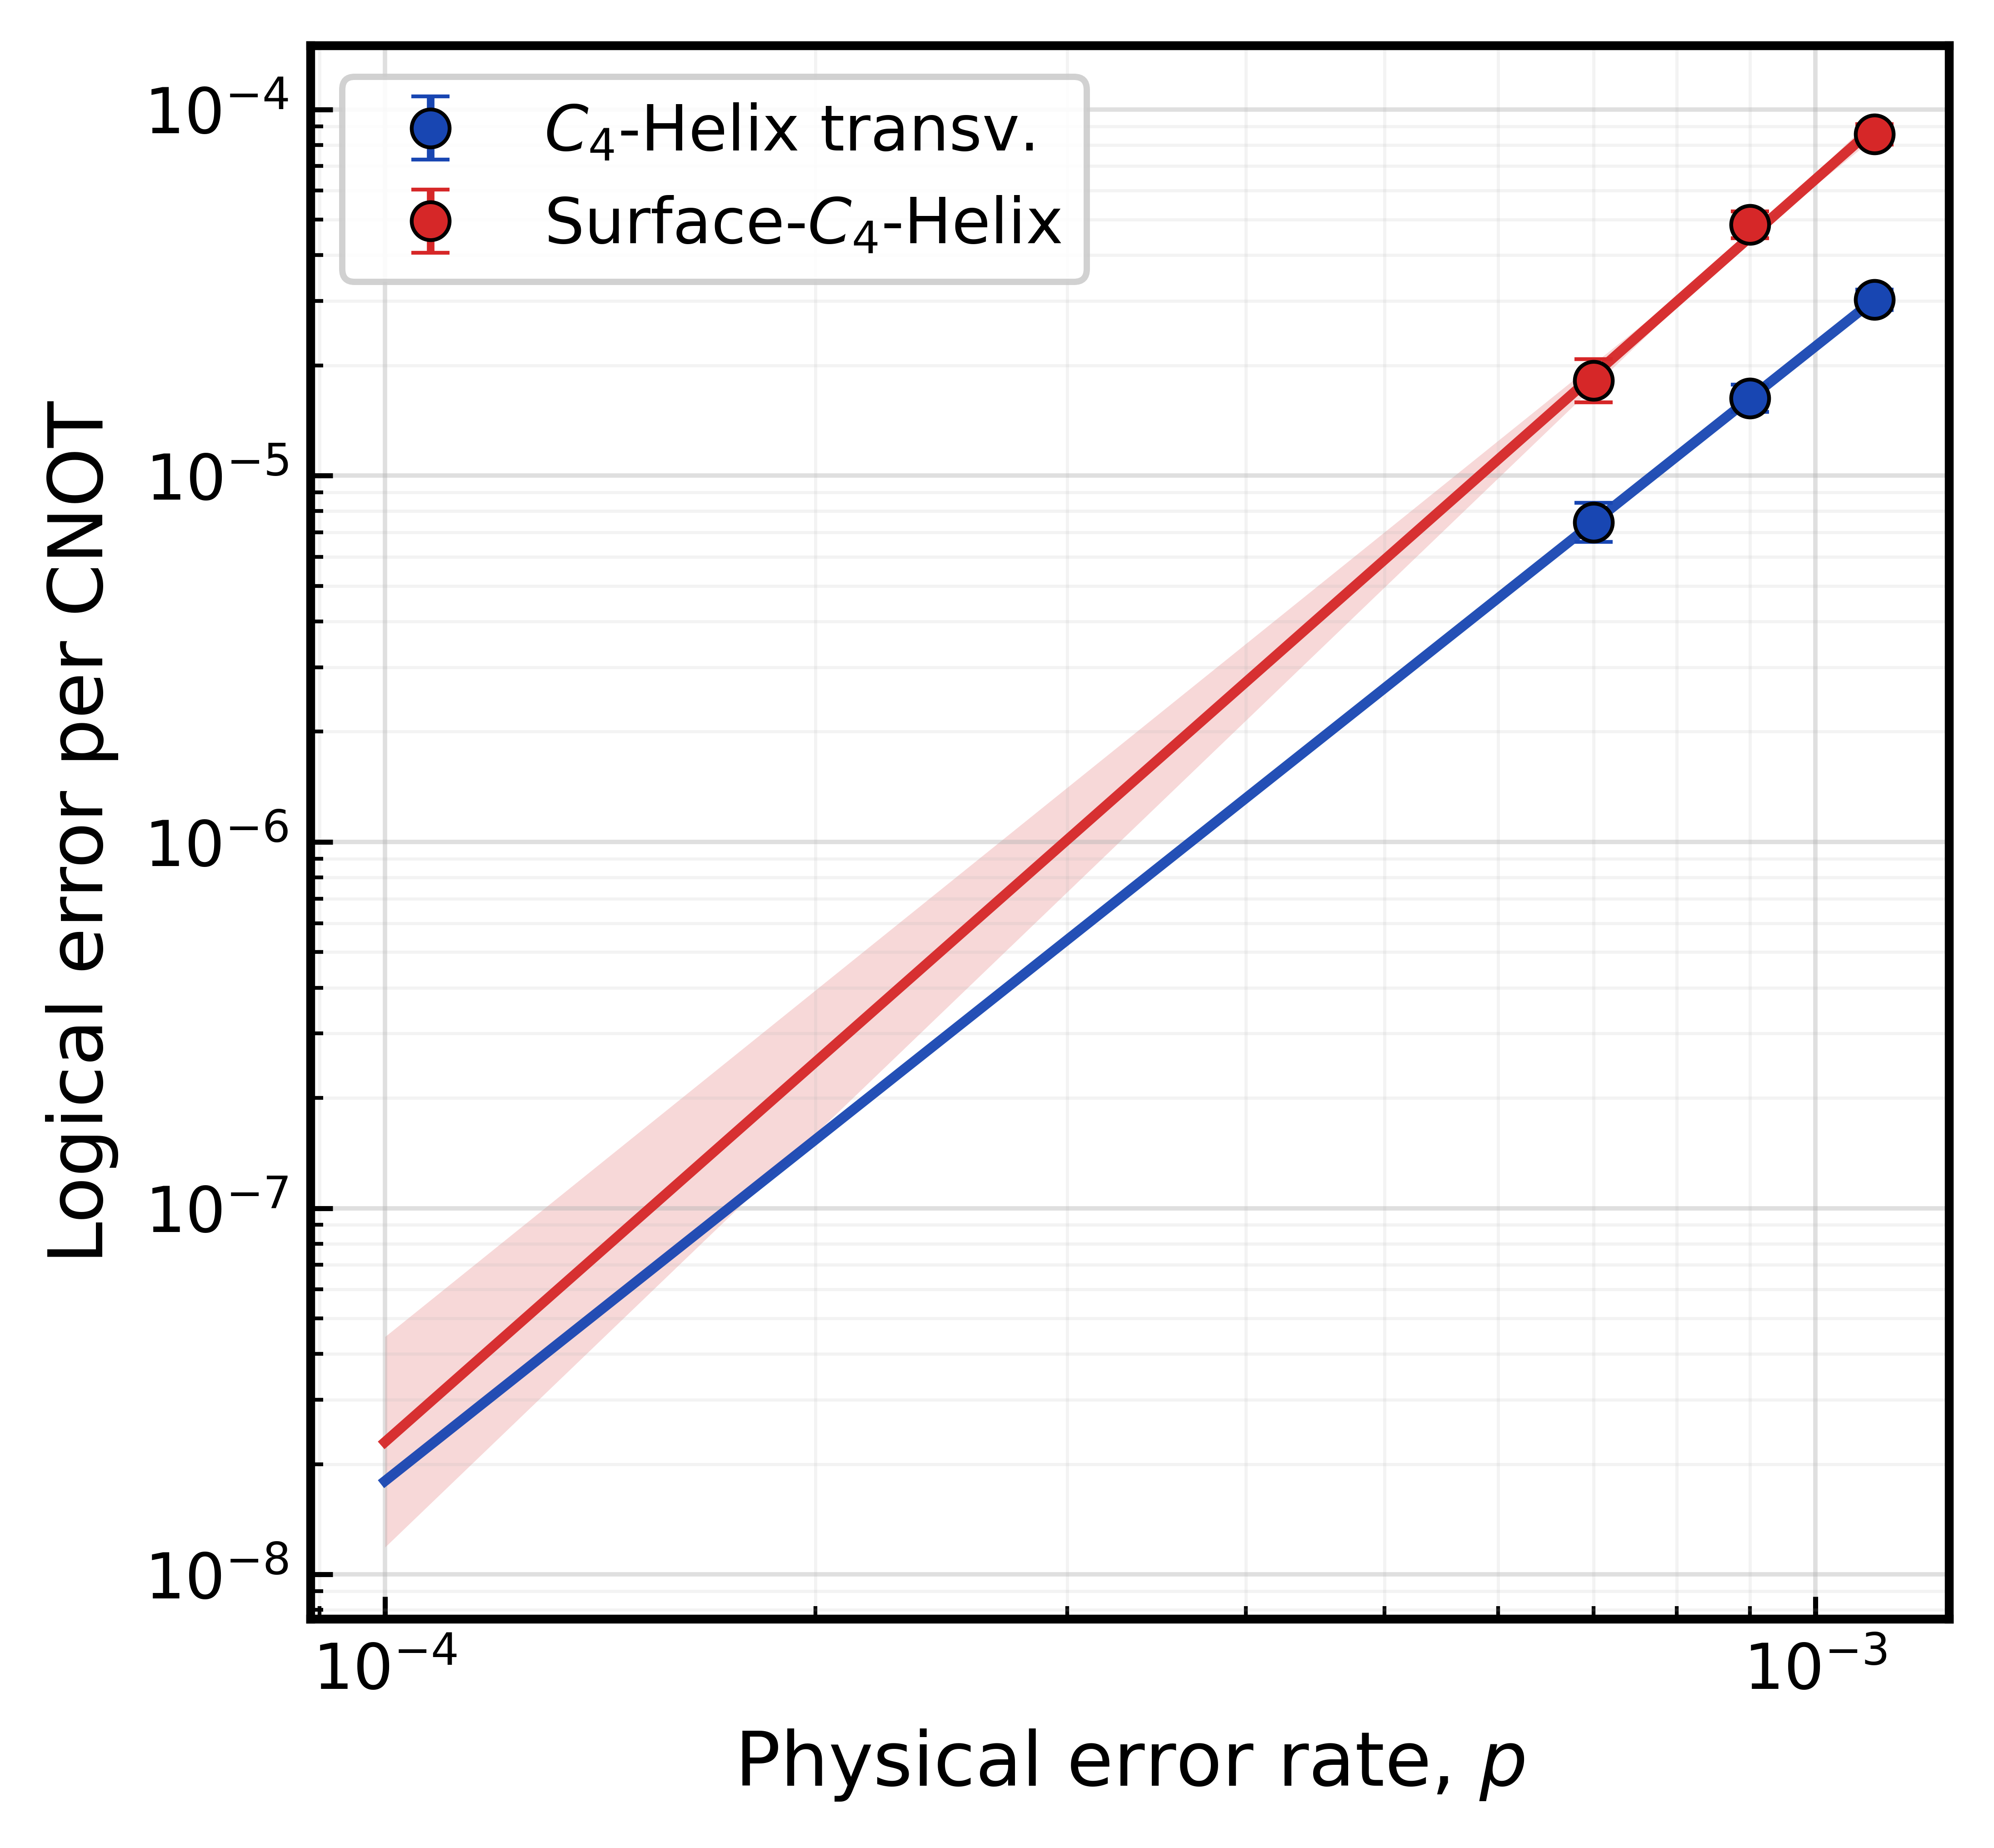
\includegraphics[width=0.85\linewidth]{figures/cnot_compare.png}
    \caption{\textbf{Simulation of a homomorphic CNOT via chain maps.} A depth-2, distance-5 homomorphic CNOT from the distance-5 surface code to the first logical qubit of the \chelix\ code, compared with transversal CNOTs in the \chelix\ code. The full experiment consists of 6 transversal/homomorphic CNOT gates interleaved with QEC cycles on each code. Dashed lines indicate power-law fits. Shaded areas indicate 95\% Wilson confidence intervals.}
    \label{fig:two-blocks}
\end{figure}

We finally simulate inter-block and inter-code operations in the \chelix\ architecture. Since the \chelix\ code is a CSS code, it has a transversal CNOT gate in which 20 pairwise physical CNOT gates between two codeblocks implements two logical CNOT gates. We perform 6 transversal CNOT gates interleaved with QEC cycles on both codeblocks, and then we destructively measure in the basis in which we prepared them. As a comparison, we simulate the chain map described in Section~\ref{sec:ghz} which performs a logical CNOT between the distance-5 surface code and the first logical qubit of the \chelix\ code. We again perform 6 homomorphic CNOT gates interleaved with QEC cycles on both codes and destructively measure in the $Z$ basis before decoding over the entire circuit. The results are shown in Fig.~\ref{fig:two-blocks} which shows both logical gates obtaining a scaling exponent near 3, as expected. We make the interesting note that performing forced-gap postselection on this homomorphic CNOT circuit only yields an improvement in the logical error rate by about a factor of 2, whereas applying it in the memory, intrablock logic, and transversal CNOT settings is able to suppress logical error rates by up to two orders of magnitude. This weaker postselection benefit is consistent with the minimum failing-fault order of the distance-5 surface code: weight-3 faults can already produce competing logical classes, leaving less confidence separation for forced-gap postselection to exploit; and so logical error rates in this chain map are inherently limited by the surface code. 

% \bibliography{bibliography}